% =====================================================================
% BMED365 (Spring 2027) — Lab 4: Kiwi 7T MRI Seed Segmentation Challenge
% Companion Guide: Promptable Vision Foundation Models on 7T MRI
% Compile with: pdflatex promptable-foundation-models.tex (run twice)
% =====================================================================
\documentclass[10.5pt,a4paper]{article}

\usepackage[utf8]{inputenc}
\usepackage[T1]{fontenc}
\usepackage[english]{babel}
\usepackage{lmodern}
\usepackage{microtype}
\usepackage{graphicx}
\usepackage{booktabs}
\usepackage{tabularx}
\usepackage{array}
\usepackage{colortbl}
\usepackage{xcolor}
\usepackage{amsmath,amssymb}
\usepackage{enumitem}
\usepackage[margin=1.9cm,headheight=14pt]{geometry}
\usepackage{fancyhdr}
\usepackage{titlesec}
\usepackage[most]{tcolorbox}
\usepackage{listings}
\usepackage{float}
\usepackage{tikz}
\usetikzlibrary{arrows.meta,positioning,shapes.geometric,fit,backgrounds,calc}
\usepackage{hyperref}

% =====================================================================
% COLORS & HYPERREF (UiB / BMED365 House Style)
% =====================================================================
\definecolor{uibblue}{RGB}{0, 61, 115}
\definecolor{uibred}{RGB}{175, 28, 44}
\definecolor{kiwigreen}{RGB}{27, 138, 90}
\definecolor{amberwarn}{RGB}{195, 110, 0}
\definecolor{lightgray}{RGB}{246, 248, 250}
\definecolor{rowalt}{RGB}{242, 246, 251}
\definecolor{codebg}{RGB}{248, 249, 251}
\definecolor{codekw}{RGB}{0, 75, 145}
\definecolor{codestr}{RGB}{155, 35, 45}
\definecolor{codecmt}{RGB}{95, 105, 115}

\hypersetup{
    colorlinks=true,
    linkcolor=uibblue,
    citecolor=uibblue,
    urlcolor=uibred,
    pdftitle={Promptable Vision Foundation Models on the 7T MRI Kiwi Challenge (BMED365 Spring 2027)},
    pdfauthor={Arvid Lundervold (UiB / MMIV) -- BMED365 Spring 2027}
}

% =====================================================================
% TYPOGRAPHY, HEADERS & CALLOUT BOXES
% =====================================================================
\setlength{\parindent}{0pt}
\setlength{\parskip}{0.45em}
\setlist[itemize]{topsep=2pt,itemsep=2pt,leftmargin=1.4em}
\setlist[enumerate]{topsep=2pt,itemsep=2pt,leftmargin=1.6em}

\newcolumntype{L}[1]{>{\raggedright\arraybackslash}p{#1}}
\newcolumntype{C}[1]{>{\centering\arraybackslash}p{#1}}
\newcolumntype{R}[1]{>{\raggedleft\arraybackslash}p{#1}}
\newcolumntype{Y}{>{\raggedright\arraybackslash}X}

\titleformat{\section}{\Large\bfseries\color{uibblue}}{\thesection}{0.7em}{}[\vspace{1pt}\titlerule]
\titleformat{\subsection}{\large\bfseries\color{uibblue!88!black}}{\thesubsection}{0.6em}{}
\titleformat{\subsubsection}{\normalsize\bfseries\color{uibblue!75!black}}{\thesubsubsection}{0.5em}{}
\titlespacing*{\section}{0pt}{1.15em}{0.45em}
\titlespacing*{\subsection}{0pt}{0.85em}{0.3em}

\pagestyle{fancy}
\fancyhf{}
\fancyhead[L]{\footnotesize\textcolor{gray}{BMED365 (Spring 2027) $\cdot$ Lab 4: Kiwi 7T MRI Seed Challenge}}
\fancyhead[R]{\footnotesize\textcolor{gray}{Promptable Vision Foundation Models}}
\fancyfoot[L]{\footnotesize\textcolor{gray}{University of Bergen \& MMIV $\cdot$ CC BY-SA 4.0}}
\fancyfoot[R]{\footnotesize\textcolor{gray}{Page \thepage}}
\renewcommand{\headrulewidth}{0.4pt}
\renewcommand{\footrulewidth}{0.2pt}

\newtcolorbox{infobox}[1][]{
    enhanced,
    colback=lightgray, colframe=uibblue,
    fonttitle=\bfseries\small, title=#1,
    boxrule=0.6pt, arc=2.5pt, left=7pt, right=7pt, top=5pt, bottom=5pt
}

\newtcolorbox{warningbox}[1][]{
    enhanced,
    colback=uibred!4, colframe=uibred,
    fonttitle=\bfseries\small, title=#1,
    boxrule=0.6pt, arc=2.5pt, left=7pt, right=7pt, top=5pt, bottom=5pt
}

\newtcolorbox{qabox}[1][]{
    enhanced,
    colback=kiwigreen!5, colframe=kiwigreen!85!black,
    fonttitle=\bfseries\small, title=#1,
    boxrule=0.6pt, arc=2.5pt, left=7pt, right=7pt, top=5pt, bottom=5pt
}

\lstdefinestyle{pybmed}{
    language=Python,
    backgroundcolor=\color{codebg},
    basicstyle=\ttfamily\scriptsize,
    keywordstyle=\bfseries\color{codekw},
    stringstyle=\color{codestr},
    commentstyle=\itshape\color{codecmt},
    showstringspaces=false,
    breaklines=true,
    breakatwhitespace=true,
    frame=single,
    rulecolor=\color{uibblue!30},
    framesep=4pt,
    xleftmargin=3pt,
    xrightmargin=3pt,
    columns=fullflexible,
    keepspaces=true,
    upquote=true
}

% =====================================================================
% DOCUMENT START
% =====================================================================
\begin{document}

% Title Banner
\begin{tcolorbox}[enhanced, colback=uibblue!6, colframe=uibblue, boxrule=1.0pt, arc=3pt, left=10pt, right=10pt, top=9pt, bottom=9pt]
{\LARGE\bfseries\color{uibblue} Promptable Vision Foundation Models on the 7T MRI Kiwi Challenge}\\[4pt]
{\normalsize\bfseries Companion Methodological \& Didactic Guide for \texttt{Lab4-Comp-Imag/Kiwi-challenge}}\\[3pt]
{\small \textbf{Course:} BMED365 --- Computational Imaging, Modeling and AI in Biomedicine (Spring 2027), University of Bergen \& MMIV\\
\textbf{Coordinator:} Arvid Lundervold \quad$\cdot$\quad \textbf{Environment:} \texttt{bmed365-2027} (\texttt{uv}, Python 3.12, \texttt{transformers >= 4.56}) \& Google Colab\\[3pt]
\textbf{Companion Resources:} \href{https://github.com/arvidl/BMED365-2027/blob/main/Lab4-Comp-Imag/Kiwi-challenge/notebooks/05-kiwi-promptable-foundation-models.ipynb}{Notebook \texttt{05} (GitHub)} $\;\vert\;$ \href{https://colab.research.google.com/github/arvidl/BMED365-2027/blob/main/Lab4-Comp-Imag/Kiwi-challenge/notebooks/05-kiwi-promptable-foundation-models.ipynb}{Open Notebook \texttt{05} in Google Colab} $\;\vert\;$ \href{https://github.com/arvidl/BMED365-2027/blob/main/Lab4-Comp-Imag/Kiwi-challenge/docs/promptable-foundation-models.md}{Markdown Version}}
\end{tcolorbox}

\vspace{-2pt}
{\small\tableofcontents}
\vspace{4pt}
\hrule
\vspace{6pt}

% =====================================================================
% SECTION 1: NON-TECHNICAL INTRODUCTION & VISUAL INTUITION
% =====================================================================
\section{A Non-Technical Introduction: Big Ideas, Definitions \& Visual Intuition}

\begin{infobox}[Who This Section Is For (Start Here!)]
The rest of this guide dives into tensor shapes, Vision Transformer physics, and reproducible PyTorch code. Before touching a single formula, this opening section builds a \textbf{plain-English mental model} of every concept, model family, and evaluation metric you will encounter --- written for biomedicine and health-science master's students with moderate math background.
\end{infobox}

\subsection{Why Should a Biomedical Scientist Care?}

Imagine you are a radiologist or biomedical researcher looking at a high-resolution 3D MRI scan of a patient's brain --- or, in our course benchmark, an intact kiwifruit scanned at 7 Tesla. You need to answer two seemingly simple clinical questions: \textbf{``How many tiny spots (microbleeds, multiple-sclerosis plaques, cell nuclei, or kiwi seeds) are inside this 3D organ?''} and \textbf{``What percentage of the organ's volume do they occupy?''}

For the past decade, answering that question with AI meant collecting hundreds of painstakingly hand-traced 3D scans, training a specialized neural network (such as a \texttt{3D U-Net}) from scratch for that exact scanner, and starting all over again whenever the hospital bought a new scanner or studied a new disease.

Since 2023, \textbf{Promptable Vision Foundation Models} --- led by Meta's \textbf{Segment Anything Model (\texttt{SAM})} and its 2024--2026 successors (\texttt{SAM 2.1}, \texttt{MedSAM}, \texttt{MedSAM2}, \texttt{MicroSAM}, \texttt{nnInteractive}, and \texttt{SAM 3}) --- have flipped that workflow upside down. Instead of training a bespoke model from scratch, you start with one massive, general-purpose visual brain that has already studied millions of images, and you \textbf{steer it on the fly} by pointing at an object with a mouse click, a rough box, or even a text phrase.

\subsection{Visual Intuition: Three Key Ideas Before Any Equations}

\begin{figure}[H]
\centering
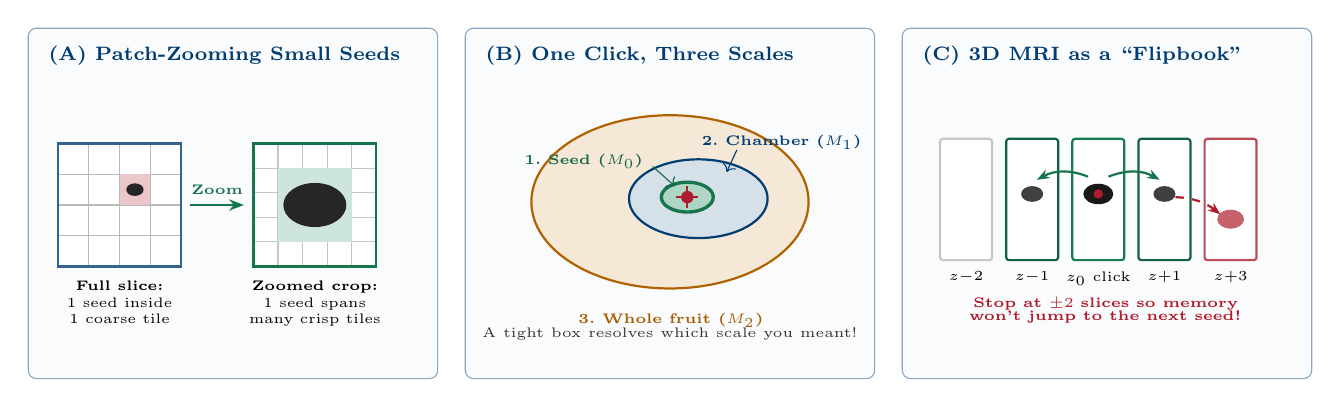
\begin{tikzpicture}[
    font=\scriptsize,
    panel/.style={rectangle, rounded corners=3pt, draw=uibblue!45, fill=lightgray!55, inner sep=4pt, minimum width=5.20cm, minimum height=4.45cm}
]
% --- PANEL A: Patch-Zooming ---
\node[panel] (pA) at (0,0) {};
\node[anchor=north west, font=\scriptsize\bfseries\color{uibblue}] at ([xshift=4pt,yshift=-3pt]pA.north west) {(A) Patch-Zooming Small Seeds};

% Left mini-grid (Full FOV: 4x4 coarse grid, tiny seed inside 1 cell)
\begin{scope}[shift={(-2.22,-0.80)}]
    \fill[white] (0,0) rectangle (1.56,1.56);
    \draw[step=0.39, gray!55, thin] (0,0) grid (1.56,1.56);
    \fill[uibred!25] (0.78,0.78) rectangle (1.17,1.17);
    \fill[black!85] (0.975,0.975) ellipse (0.11 and 0.08);
    \draw[uibblue!80, thick] (0,0) rectangle (1.56,1.56);
    \node[below, align=center, font=\tiny] at (0.78,-0.06) {\textbf{Full slice:}\\1 seed inside\\1 coarse tile};
\end{scope}

% Arrow
\draw[-{Stealth[length=1.9mm]}, thick, color=kiwigreen!85!black] (-0.54,-0.02) -- (0.14,-0.02) node[midway, above, font=\tiny\bfseries\color{kiwigreen!80!black}] {Zoom};

% Right mini-grid (Zoomed ROI: seed spans 3x3 tiles)
\begin{scope}[shift={(0.26,-0.80)}]
    \fill[white] (0,0) rectangle (1.56,1.56);
    \draw[step=0.312, gray!45, thin] (0,0) grid (1.56,1.56);
    \fill[kiwigreen!22] (0.312,0.312) rectangle (1.248,1.248);
    \fill[black!85] (0.78,0.78) ellipse (0.40 and 0.28);
    \draw[kiwigreen!85!black, thick] (0,0) rectangle (1.56,1.56);
    \node[below, align=center, font=\tiny] at (0.78,-0.06) {\textbf{Zoomed crop:}\\1 seed spans\\many crisp tiles};
\end{scope}

% --- PANEL B: Part-Whole Ambiguity ---
\node[panel] (pB) at (5.55,0) {};
\node[anchor=north west, font=\scriptsize\bfseries\color{uibblue}] at ([xshift=4pt,yshift=-3pt]pB.north west) {(B) One Click, Three Scales};

\begin{scope}[shift={(5.55,0.02)}]
    % Whole fruit (M2)
    \fill[amberwarn!16, draw=amberwarn!90!black, thick] (0,0) ellipse (1.76 and 1.10);
    % Locule chamber (M1)
    \fill[uibblue!16, draw=uibblue, thick] (0.36,0.04) ellipse (0.88 and 0.50);
    % Single seed (M0)
    \fill[kiwigreen!35, draw=kiwigreen!85!black, very thick] (0.22,0.06) ellipse (0.33 and 0.19);
    % Click marker
    \node[circle, fill=uibred, inner sep=1.6pt] (clk) at (0.22,0.06) {};
    \draw[uibred, thick] (0.08,0.06) -- (0.36,0.06) (0.22,-0.08) -- (0.22,0.20);
    % Labels
    \node[font=\tiny\bfseries, color=kiwigreen!75!black, anchor=east] at (-0.22,0.52) {1.\ Seed ($M_0$)};
    \draw[->, thin, color=kiwigreen!75!black] (-0.22,0.45) -- (0.06,0.20);
    \node[font=\tiny\bfseries, color=uibblue, anchor=west] at (0.28,0.76) {2.\ Chamber ($M_1$)};
    \draw[->, thin, color=uibblue] (0.85,0.66) -- (0.72,0.38);
    \node[font=\tiny\bfseries, color=amberwarn!85!black, align=center, text width=4.8cm] at (0,-1.58) {3.\ Whole fruit ($M_2$)\\[-1pt]\normalfont\color{black!80}A tight box resolves which scale you meant!};
\end{scope}

% --- PANEL C: 3D Flipbook Memory ---
\node[panel] (pC) at (11.10,0) {};
\node[anchor=north west, font=\scriptsize\bfseries\color{uibblue}] at ([xshift=4pt,yshift=-3pt]pC.north west) {(C) 3D MRI as a ``Flipbook''};

\begin{scope}[shift={(8.98,-0.88)}]
    % Draw 5 stacked slices
    \foreach \i/\lbl/\col in {0/$z{-}2$/gray!45, 1/$z{-}1$/kiwigreen!70!black, 2/$z_0$ click/kiwigreen!90!black, 3/$z{+}1$/kiwigreen!70!black, 4/$z{+}3$/uibred!80}{
        \pgfmathsetmacro{\xoff}{\i*0.84}
        \fill[white, draw=\col, thick, rounded corners=1pt] (\xoff,0.16) rectangle (\xoff+0.66,1.70);
        \node[font=\tiny, below] at (\xoff+0.33,0.14) {\lbl};
    }
    % Seed 1 across z-1, z0, z+1
    \fill[black!75] (1.17,1.00) ellipse (0.14 and 0.10);
    \fill[black!90] (2.01,1.00) ellipse (0.19 and 0.13);
    \node[circle, fill=uibred, inner sep=1.2pt] at (2.01,1.00) {};
    \fill[black!75] (2.85,1.00) ellipse (0.14 and 0.10);
    % Different seed behind on z+3
    \fill[uibred!70] (3.69,0.68) ellipse (0.17 and 0.12);
    % Good tracking arrows
    \draw[-{Stealth[length=1.6mm]}, thick, color=kiwigreen!85!black] (1.88,1.22) to[bend right=25] (1.23,1.18);
    \draw[-{Stealth[length=1.6mm]}, thick, color=kiwigreen!85!black] (2.14,1.22) to[bend left=25] (2.79,1.18);
    % Bad jump arrow
    \draw[-{Stealth[length=1.6mm]}, thick, dashed, color=uibred] (2.99,0.96) to[bend left=18] (3.56,0.74);
    \node[font=\tiny\bfseries, color=uibred, align=center, text width=4.8cm] at (2.10,-0.48) {Stop at $\pm 2$ slices so memory\\[-1pt]won't jump to the next seed!};
\end{scope}
\end{tikzpicture}
\caption{Visual intuition for the three central ideas behind promptable vision foundation models on 3D medical scans: (A)~Patch-Zooming rescues small lesions from coarse Transformer grids; (B)~one click admits nested part--whole interpretations; (C)~slice-by-slice video memory tracks a 3D seed like a flipbook, but needs a physical depth limit to avoid jumping onto neighboring seeds.}
\label{fig:nontech-sam-intuition}
\end{figure}

\newpage
\subsection{Core Concepts Defined in Plain English}

\begin{table}[H]
\centering
\footnotesize
\renewcommand{\arraystretch}{1.18}
\rowcolors{2}{white}{rowalt}
\begin{tabularx}{\textwidth}{L{3.55cm} Y}
\toprule
\rowcolor{uibblue!14}
\textbf{Concept / Term} & \textbf{Plain-English Meaning \& Everyday / Clinical Analogy} \\
\midrule
\textbf{Semantic vs.\ Instance Segmentation} & \textbf{Semantic segmentation} is like coloring every person in a crowd photo blue: you know where ``crowd'' pixels are, but touching people blur into one blob. \textbf{Instance segmentation} puts a separate numbered name tag on \emph{each individual person} (or each individual kiwi seed / MS plaque) so you can count them accurately. \\
\textbf{Foundation Model \& ``Zero-Shot''} & A large AI model pre-trained on a vast, diverse library of images so it develops broad visual common sense (edges, shapes, textures, depth). \textbf{Zero-shot} means asking it to segment a brand-new type of scan (like our 7T kiwifruit MRI) \emph{without} retraining it on any labeled kiwi examples first. \\
\textbf{Prompting (Click, Negative Click, Box, Text)} & How you tell the model \emph{which} object you want outlined: a \textbf{positive click} says ``include this spot''; a \textbf{negative click} says ``exclude this background''; a \textbf{bounding box} draws a loose frame around the target (like a radiologist's caliper); a \textbf{text prompt} (\texttt{SAM 3}) describes it in words. \\
\textbf{Vision Transformer (\texttt{ViT}) \& Patch Tokens} & Rather than inspecting one tiny pixel at a time like a magnifying glass (the way older convolutional networks work), a Vision Transformer slices an image into a checkerboard of small square tiles called \textbf{patches} (tokens) and lets every tile compare notes with every other tile simultaneously (\emph{self-attention}). \\
\textbf{Patch-Zooming \& Hierarchical (\texttt{Hiera}) Backbone} & If a target object (like a 1\,mm microbleed or kiwi seed) is smaller than a single checkerboard tile, the Transformer barely sees it. \textbf{Patch-Zooming} crops and enlarges a smaller region before slicing it into tiles so the seed fills several tiles. A \textbf{hierarchical backbone} (\texttt{Hiera} in \texttt{SAM 2.1}) keeps both a wide overview map and fine high-resolution detail maps at the same time. \\
\textbf{Part--Whole Ambiguity (Multi-Mask Output)} & Clicking once inside a kiwi seed is inherently ambiguous: did you mean \emph{this one seed}, \emph{the whole chamber around it}, or \emph{the entire fruit}? (Just as clicking inside a brain tumor could mean the necrotic core, the enhancing ring, or the whole swelling.) \texttt{SAM} handles this by proposing \textbf{three nested guesses} (small, medium, large) along with its own confidence score for each. \\
\textbf{3D Slice Memory (\emph{``Flipbook''} Tracking)} & Most foundation models were trained on 2D photos or videos, not 3D medical volumes. \texttt{SAM 2.1} and \texttt{MedSAM2} treat a 3D MRI stack like a \textbf{flipbook movie}: you click a seed on one middle slice, and the model uses a short-term \textbf{memory bank} to follow that same seed upward and downward through neighboring slices. \\
\textbf{Occlusion \& Confidence Scores} & As the flipbook tracker moves past the top or bottom tip of a seed, it must know when to stop. \texttt{SAM 2.1} outputs an \textbf{object-presence score} (``is the seed still here, or has it ended?'') and a \textbf{predicted IoU score} (``how sharp and trustworthy is my outline?''). \\
\textbf{``Stuff'' vs.\ ``Things'' \& Neurosymbolic Guardrails} & Large background regions (\emph{peel, fruit flesh, central core}) are \textbf{Stuff}; small countable objects (\emph{seeds, lesions}) are \textbf{Things}. Asking \texttt{SAM} to ``segment everything'' mostly finds easy Stuff. A \textbf{neurosymbolic pipeline} pairs simple biological rules (``seeds live only in the inner seed ring and look dark in bright gel'') with neural mask tracing so the computer prompts itself reliably. \\
\textbf{How We Grade Masks (\texttt{IoU}, \texttt{Dice}, \texttt{PQ})} & \textbf{IoU} and \textbf{Dice} measure overlap between the AI's painted region and the true outline (0 = miss, 1 = perfect). However, merging two touching seeds can still score a high Dice! \textbf{Panoptic Quality (\texttt{PQ})} fixes this by multiplying \emph{how cleanly matched seeds are traced} (\textbf{Segmentation Quality, \texttt{SQ}}) by \emph{what fraction of seeds were found 1-to-1 without merges or splits} (\textbf{Recognition Quality, \texttt{RQ}}). \\
\bottomrule
\end{tabularx}
\caption{Plain-English definitions of the core concepts appearing throughout this guide.}
\label{tab:nontech-defs}
\end{table}

\subsection{Meet the Model Families (No Jargon Required)}

Several model names appear throughout this guide. Here is how they fit together as a family tree:
\begin{itemize}
    \item \textbf{\texttt{SAM 1} \& \texttt{SAM-HQ} (2023):} Meta's original ``click-anything'' 2D photo segmenter (\texttt{SAM 1}), plus a sharpness upgrade (\texttt{SAM-HQ}) that adds fine edge detail. Great on everyday photos, but works only on one 2D slice at a time.
    \item \textbf{\texttt{MedSAM} (2024):} The first major medical adaptation of \texttt{SAM 1}, retrained on over 1.5 million clinical CT, MRI, and ultrasound masks. Crucially, it was trained almost exclusively with \textbf{bounding boxes} (matching clinical measurement calipers), so it works poorly if you give it only a single dot click.
    \item \textbf{\texttt{SAM 2} / \texttt{SAM 2.1} (2024--2025):} Meta's next-generation model with two breakthroughs for medical imaging: (1)~a sharper multi-scale encoder (\texttt{Hiera}) that sees smaller objects much better, and (2)~a \textbf{video memory bank} that lets a single click propagate through a 3D MRI slice stack. It is open, fast, and runs directly on laptops and Google Colab.
    \item \textbf{\texttt{MedSAM2} \& \texttt{MicroSAM} (2025):} Domain specialists built on the \texttt{SAM} family --- \texttt{MedSAM2} adapts \texttt{SAM 2.1}'s 3D slice tracking to clinical organs and tumors, while \texttt{MicroSAM} specializes in tightly packed cells and organelles under microscopes (very similar to packed kiwi seeds!).
    \item \textbf{\texttt{nnInteractive} (2025) \& \texttt{SAM 3} (2025--2026):} \texttt{nnInteractive} (from the German Cancer Research Center, DKFZ) ditches the 2D-video shortcut altogether and operates natively in true 3D on an NVIDIA GPU (supporting clicks, boxes, scribbles, and 3D lassos). \texttt{SAM 3} adds natural-language concept prompts (e.g., typing \emph{``dark oval seed''}) alongside clicks and video tracking.
\end{itemize}

\subsection{Recommended Starting Resources (Reviews, Visual Guides, Repos, Videos \& Podcasts)}

Before or alongside the technical sections below, these curated educational links build intuition without heavy math:

\begin{table}[H]
\centering
\scriptsize
\renewcommand{\arraystretch}{1.20}
\rowcolors{2}{white}{rowalt}
\begin{tabularx}{\textwidth}{L{2.55cm} Y}
\toprule
\rowcolor{uibblue!14}
\textbf{Format} & \textbf{Curated Learning Resource (Clickable)} \\
\midrule
\textbf{Non-Technical Review Papers} &
$\bullet$ \href{https://doi.org/10.1038/s41586-023-05881-4}{\textbf{Moor et al., \emph{Nature} (2023)}} --- \emph{Foundation models for generalist medical AI} (accessible big-picture vision for clinicians \& biologists). \newline
$\bullet$ \href{https://doi.org/10.1038/s41592-023-02151-z}{\textbf{Maier-Hein et al., \emph{Nature Methods} (2024)}} --- \emph{Metrics reloaded} (clear visual guide to why Dice fails when counting touching objects). \newline
$\bullet$ \href{https://doi.org/10.1038/s41467-024-44824-z}{\textbf{Ma et al., \emph{Nature Communications} (2024)}} (\texttt{MedSAM}) \& \href{https://doi.org/10.1038/s41592-024-02580-4}{\textbf{Archit et al., \emph{Nature Methods} (2025)}} (\texttt{MicroSAM}). \\
\textbf{Interactive Demos \& Visual Tutorials} &
$\bullet$ \href{https://sam2.metademolab.com/}{\textbf{Meta AI SAM 2 Interactive Web Demo}} --- click and track objects live in your browser (2 minutes builds immediate intuition!). \newline
$\bullet$ \href{https://ai.meta.com/blog/segment-anything-model-2/}{\textbf{Meta AI Blog: Introducing SAM 2}} --- plain-English overview with animations of streaming memory. \newline
$\bullet$ \href{https://jalammar.github.io/illustrated-transformer/}{\textbf{Jay Alammar: \emph{The Illustrated Transformer}}} --- the gold-standard visual walkthrough of attention and tokens. \newline
$\bullet$ \href{https://huggingface.co/docs/transformers/model_doc/sam2}{\textbf{Hugging Face \texttt{transformers} SAM 2 Docs}} --- beginner-friendly Python usage guide for the exact API used in Notebook~\texttt{05}. \\
\textbf{Open-Source GitHub Repos} &
\href{https://github.com/facebookresearch/sam2}{\texttt{facebookresearch/sam2}} $\;\cdot\;$
\href{https://github.com/bowang-lab/MedSAM}{\texttt{bowang-lab/MedSAM}} $\;\cdot\;$
\href{https://github.com/bowang-lab/MedSAM2}{\texttt{bowang-lab/MedSAM2}} $\;\cdot\;$
\href{https://github.com/computational-cell-analytics/micro-sam}{\texttt{computational-cell-analytics/micro-sam}} $\;\cdot\;$
\href{https://github.com/MIC-DKFZ/nnInteractive}{\texttt{MIC-DKFZ/nnInteractive}} \\
\textbf{Videos \& Podcasts} &
$\bullet$ \href{https://www.3blue1brown.com/lessons/attention}{\textbf{3Blue1Brown: \emph{Attention in Transformers, Visually Explained}}} (\href{https://www.youtube.com/watch?v=eMlx5fFNoYc}{YouTube video}, $\sim 26\text{ min}$) --- best animated explanation of how Transformers think. \newline
$\bullet$ \href{https://www.youtube.com/watch?v=1d3L0g0GzEE}{\textbf{RSNA \emph{Radiology: AI} Feature}} --- \emph{``Foundation Models in Radiology: What, How, Why, and Why Not?''} \newline
$\bullet$ \href{https://ai-podcast.nejm.org/}{\textbf{NEJM AI Grand Rounds Podcast}} --- clinician-scientist conversations on medical foundation models and real-world validation. \\
\bottomrule
\end{tabularx}
\caption{Curated non-technical readings, interactive demos, code repositories, videos, and podcasts to pair with this guide.}
\label{tab:nontech-sam-resources}
\end{table}

\newpage
% =====================================================================
% SECTION 2: LLM TO VISION FOUNDATION MODEL BRIDGE
% =====================================================================
\section{From Chatbot LLMs (Lab 3) to Promptable Vision Foundation Models (Lab 4)}

If you have worked with Large Language Models (\texttt{LLMs}) such as ChatGPT, Claude, or Gemini in \href{https://github.com/arvidl/BMED365-2027/tree/main/Lab3-GenAI-LLM}{\textbf{Lab 3 (\texttt{Lab3-GenAI-LLM})}}, you already know 80\% of the mental model behind a \textbf{Promptable Vision Foundation Model} such as \texttt{SAM}, \texttt{MedSAM}, or \texttt{SAM 2.1}. Both are built on the exact same \textbf{Transformer} primitives --- \emph{tokens}, \emph{high-dimensional embedding vectors}, \emph{positional encodings}, and \emph{attention} --- adapted from 1D text sequences to 2D and 3D biomedical images.

\subsection{The Side-by-Side Rosetta Stone: Text Chatbot LLM vs.\ Promptable Segmentation Model}

\begin{table}[!ht]
\centering
\footnotesize
\renewcommand{\arraystretch}{1.22}
\rowcolors{2}{white}{rowalt}
\begin{tabularx}{\textwidth}{L{3.1cm} Y Y}
\toprule
\rowcolor{uibblue!14}
\textbf{Architectural Stage} & \textbf{Natural-Language Chatbot LLM (Lab 3)} & \textbf{Promptable Vision Foundation Model (Lab 4)} \\
\midrule
\textbf{1. Raw Context Input} & A clinical note or research paper (1D character string) & A 2D MRI slice of size $H \times W$ (rescaled to $1024 \times 1024 \times 3$), or a 3D slice stack $z = 0 \dots Z-1$ \\
\textbf{2. Tokenization} \newline \emph{(``What is a token?'')} & \textbf{Subword BPE pieces} (\texttt{tiktoken}, e.g., \texttt{"micro"}, \texttt{"bleed"} $\to$ integer token IDs) & \textbf{Non-overlapping $16 \times 16$ pixel squares (\emph{Visual Patches})}: slicing $1024 \times 1024$ into a $64 \times 64$ grid = \textbf{4,096 visual tokens} \\
\textbf{3. Token Embedding} ($\mathbf{e} \in \mathbb{R}^d$) & Vocabulary lookup table maps each token ID to a vector (e.g., $d = 4{,}096$) & A strided $16 \times 16$ 2D convolution projects the $16 \times 16 \times 3 = 768$ pixel values of each square into a \textbf{256-D visual vector} \\
\textbf{4. Positional Encoding} & \textbf{1D sequence index} (\texttt{RoPE} / sinusoids $i = 1 \dots L$) so word order is preserved & \textbf{2D spatial $(x, y)$ Fourier / rotary coordinates} added to every patch vector so the Transformer knows \emph{where} each patch sits \\
\textbf{5. Context Caching} & \textbf{KV-Cache} of a long uploaded PDF (encoded once, queried repeatedly) & \textbf{Image Encoder (\texttt{ViT} / \texttt{Hiera}) runs ONCE per slice} ($\sim 80\text{ ms}$) to cache a reusable \textbf{Image Embedding Map} $\mathcal{F} \in \mathbb{R}^{256 \times 64 \times 64}$ \\
\textbf{6. User Prompt} \newline \emph{(``How you steer it'')} & Natural-language question tokens (\texttt{"List the focal lesions"}) & \textbf{Geometric Prompt Tokens}: click $(x, y)$ (\texttt{+1} fg / \texttt{0} bg) or box corners $(x_1, y_1), (x_2, y_2)$ mapped to 256-D vectors ($< 2\text{ ms}$) \\
\textbf{7. Decoder Reasoning} & Causal self-attention over \texttt{[context + prompt]} tokens & \textbf{Two-Way Cross-Attention ($\sim 4\text{M}$ params)}: prompt tokens query image tokens \emph{and} image tokens query prompt tokens \\
\textbf{8. Output Prediction} & Linear head over vocabulary $\to$ \textbf{next-word probabilities} & Dot product between a learned \textbf{Mask Token} and upsampled pixel features $\to$ \textbf{2D Mask Logit Map} $L_m(x,y)$ + \textbf{confidence} $\widehat{\text{IoU}} \in [0,1]$ \\
\textbf{9. Multi-Turn Memory} & Chat history carried across turns $t = 1, 2, \dots$ & \textbf{Streaming Memory Bank (\texttt{Sam2VideoModel})}: encoding slice $z_0$'s mask so adjacent slices $z_0 \pm 1, \pm 2$ track the same 3D seed \\
\bottomrule
\end{tabularx}
\caption{Conceptual mapping between 1D language Transformers (Block 1, Lab 3) and 2D/3D promptable vision Transformers (Block 2, Lab 4).}
\end{table}

\subsection{Following One Click Through the Tensors (End-to-End Dataflow)}

\begin{figure}[ht!]
\centering
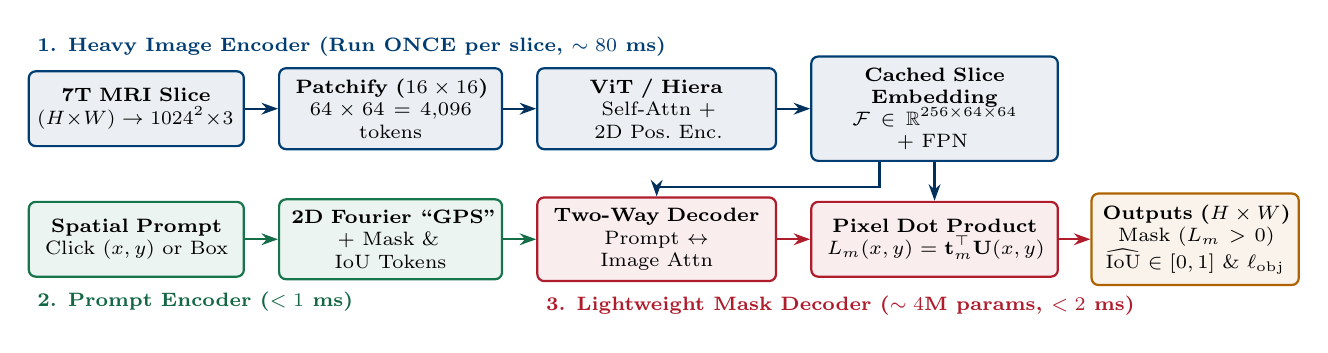
\begin{tikzpicture}[
    font=\scriptsize,
    node distance=0.35cm and 0.42cm,
    box/.style={rectangle, rounded corners=2.5pt, draw=#1, fill=#1!8, thick, align=center, inner sep=4pt, minimum height=0.95cm},
    arr/.style={-{Stealth[length=2.1mm,width=1.5mm]}, thick, draw=uibblue!80!black}
]
% Row 1: Heavy Image Encoder
\node[box=uibblue, text width=2.45cm] (img) {\textbf{7T MRI Slice}\\$(H \times W) \to 1024^2 \times 3$};
\node[box=uibblue, text width=2.55cm, right=of img] (patch) {\textbf{Patchify ($16\times 16$)}\\$64\times 64 = 4{,}096$ tokens};
\node[box=uibblue, text width=2.75cm, right=of patch] (vit) {\textbf{ViT / Hiera}\\Self-Attn + 2D Pos.\ Enc.};
\node[box=uibblue, text width=2.85cm, right=of vit] (emb) {\textbf{Cached Slice Embedding}\\$\mathcal{F} \in \mathbb{R}^{256\times 64\times 64}$ + FPN};

\draw[arr] (img) -- (patch);
\draw[arr] (patch) -- (vit);
\draw[arr] (vit) -- (emb);

% Row 2: Prompt Encoder + Decoder
\node[box=kiwigreen!85!black, text width=2.45cm, below=0.68cm of img] (prm) {\textbf{Spatial Prompt}\\Click $(x,y)$ or Box};
\node[box=kiwigreen!85!black, text width=2.55cm, right=of prm] (fourier) {\textbf{2D Fourier ``GPS''}\\+ Mask \& IoU Tokens};
\node[box=uibred, text width=2.75cm, right=of fourier] (xattn) {\textbf{Two-Way Decoder}\\Prompt $\leftrightarrow$ Image Attn};
\node[box=uibred, text width=2.85cm, right=of xattn] (dot) {\textbf{Pixel Dot Product}\\$L_m(x,y) = \mathbf{t}_m^\top \mathbf{U}(x,y)$};
\node[box=amberwarn!90!black, text width=2.35cm, right=0.40cm of dot] (out) {\textbf{Outputs ($H\times W$)}\\Mask $(L_m > 0)$\\$\widehat{\text{IoU}} \in [0,1]$ \& $\ell_{\text{obj}}$};

\draw[arr, draw=kiwigreen!80!black] (prm) -- (fourier);
\draw[arr, draw=kiwigreen!80!black] (fourier) -- (xattn);
\draw[arr] ([xshift=-0.7cm]emb.south) -- ++(0,-0.32) -| (xattn.north);
\draw[arr, draw=uibred] (xattn) -- (dot);
\draw[arr, draw=uibblue!80!black] (emb.south) -- (dot.north);
\draw[arr, draw=uibred] (dot) -- (out);

% Group labels
\node[anchor=south west, font=\scriptsize\bfseries\color{uibblue}] at ([yshift=1.5pt]img.north west) {1. Heavy Image Encoder (Run ONCE per slice, $\sim 80\text{ ms}$)};
\node[anchor=north west, font=\scriptsize\bfseries\color{kiwigreen!75!black}] at ([yshift=-1.5pt]prm.south west) {2. Prompt Encoder ($< 1\text{ ms}$)};
\node[anchor=north west, font=\scriptsize\bfseries\color{uibred}] at ([yshift=-1.5pt]xattn.south west) {3. Lightweight Mask Decoder ($\sim 4\text{M}$ params, $< 2\text{ ms}$)};
\end{tikzpicture}
\caption{End-to-end tensor dataflow inside \texttt{SAM} / \texttt{SAM 2.1}, separating one-time heavy slice encoding (top) from sub-millisecond prompt-conditioned decoding (bottom).}
\label{fig:sam-dataflow}
\end{figure}

Four concrete insights explain what happens inside Figure~\ref{fig:sam-dataflow}:
\begin{enumerate}
    \item \textbf{Why chop an image into $16 \times 16$ patches instead of treating every pixel as a token?} Self-attention scales quadratically as $\mathcal{O}(N^2)$. A $1024 \times 1024$ image contains $N = 1{,}048{,}576$ pixels, so pixel-to-pixel attention would require $N^2 \approx 1.1 \times 10^{12}$ pairwise weights per layer! Grouping pixels into $16 \times 16$ squares compresses the sequence $256\times$ to $N = 64 \times 64 = 4{,}096$ visual tokens ($N^2 \approx 1.67 \times 10^7$) --- roughly the context length of a 10-page text document in an LLM. \emph{(As we prove in Section~\ref{sec:trap1}, this exact $16 \times 16$ compression is also why 5-pixel kiwifruit seeds require Patch-Zooming!)}
    \item \textbf{How do two coordinates $(x = 21.5, y = 4.9)$ become a 256-D ``word''?} Feeding two raw floats $(x/W, y/H) \in [0, 1]^2$ into a small MLP blurs nearby positions together (\emph{spectral bias}). Instead, the \textbf{Prompt Encoder} maps $(x/W, y/H)$ through 128 multi-frequency 2D sine and cosine waves (\emph{Fourier positional encoding} --- a spatial ``GPS barcode'' from coarse whole-slice waves down to sub-pixel waves) and adds a learned role vector (\texttt{foreground click}, \texttt{background click}, or \texttt{box corner}), placing the prompt in the \textbf{exact same 256-D space} as the image patches.
    \item \textbf{An LLM outputs a word from a vocabulary --- how does a Transformer output a 2D picture?} Alongside your prompt tokens, the decoder prepends learnable readout tokens (analogous to \texttt{[CLS]}): \textbf{3 Output Mask Tokens} ($\mathbf{t}_0, \mathbf{t}_1, \mathbf{t}_2 \in \mathbb{R}^{256}$) and \textbf{1 IoU Score Token}. Via Two-Way Cross-Attention, each $\mathbf{t}_m$ becomes an \textbf{on-the-fly linear classifier weight vector} tailored to the clicked object. Meanwhile, transposed convolutions upsample the $64 \times 64$ image features (fused with $256 \times 256$ \texttt{stride-4} FPN features in \texttt{SAM 2.1}) into a per-pixel feature map $\mathbf{U}(x, y) \in \mathbb{R}^{256}$. Taking the dot product at every pixel produces the 2D foreground logit map:
    \[
        L_m(x, y) = \mathbf{t}_m^\top \, \mathbf{U}(x, y) \in \mathbb{R}, \qquad \text{Mask}_m(x, y) = \mathbb{I}\!\left[L_m(x, y) > 0\right],
    \]
    while the sibling IoU Token predicts $\widehat{\text{IoU}}_m \in [0, 1]$ (\texttt{iou\_scores}) --- the model's self-estimated boundary quality!
    \item \textbf{Why split a heavy Image Encoder from a tiny Prompt Decoder?} Because $\mathcal{F}$ does not depend on the prompt, interactive viewers (3D Slicer, Napari, or Notebook~\texttt{03b}) encode a slice \textbf{once} ($\sim 80\text{ ms}$) and decode dozens of clicks in $< 2\text{ ms}$ each. In \textbf{\texttt{SAM 2.1} (\texttt{Sam2VideoModel})}, a \textbf{Memory Encoder} fuses slice $z_0$'s features with its predicted mask into a \textbf{FIFO Memory Bank} (a visual KV-cache) so adjacent 3D slices ($z_0 \pm 1, \pm 2$) segment the rest of the 3D seed automatically.
\end{enumerate}

% =====================================================================
% SECTION 2: MOTIVATION, LEARNING OUTCOMES & GLOSSARY
% =====================================================================
\section{Why Test Vision Foundation Models on a 7T Kiwifruit MRI?}

At first glance, one might expect a foundation model trained on millions of masks to solve the \href{https://github.com/arvidl/BMED365-2027/tree/main/Lab4-Comp-Imag/Kiwi-challenge}{\textbf{Kiwi 7T MRI Seed Challenge}} effortlessly in ``zero-shot'' mode. In practice, applying a foundation model to our $256 \times 256 \times 128$ ($0.234 \times 0.234 \times 0.500\text{ mm}^3$) $T_2$-weighted RARE scan exposes \textbf{four physics, resolution, and topology traps} that appear identically when segmenting \textbf{cerebral microbleeds (\texttt{CMBs})}, \textbf{punctate multiple sclerosis (\texttt{MS}) plaques}, \textbf{micrometastases}, or \textbf{packed 3D cell nuclei}:
\begin{enumerate}
    \item \textbf{The ViT Patch-Stride Bottleneck (\emph{Micro-Object Blindness}):} A single kiwifruit seed spans only $4\text{--}5 \times 7\text{--}8$ pixels in-plane --- roughly \emph{one} $16 \times 16$ ViT token when a full $256 \times 256$ slice is encoded directly.
    \item \textbf{Prompt-Modality \& Scale-Ambiguity Mismatch:} Medical checkpoints like \texttt{MedSAM} were fine-tuned exclusively on \emph{bounding boxes} around macro-organs/tumors and fail on point clicks, whereas single clicks in \texttt{SAM 2.1} trigger nested part--whole ambiguity (\emph{seed} vs.\ \emph{locule} vs.\ \emph{whole berry}).
    \item \textbf{Anisotropic 2D-to-3D Slice Memory Drift:} Treating axial slices $z = 0 \dots 127$ as video frames (as in \texttt{Sam2VideoModel} and \texttt{MedSAM2}) propagates masks across $z$, \textbf{but} at $0.50\text{ mm}$ slice thickness ($2.1\times$ coarser than in-plane), unbounded memory jumps across seed poles and merges stacked neighbors along $z$.
    \item \textbf{``Who Prompts the Prompter?'' (\emph{Stuff vs.\ Things \& Anatomical Priors}):} Unprompted grids segment macroscopic \textbf{Stuff} (\emph{peel}, \emph{pericarp}, \emph{central columella}) while missing tiny \textbf{Things} (\emph{seeds}); conversely, naive automated point proposals fire on speckled outer-cortex parenchyma unless gated by neurosymbolic anatomical priors and confidence tokens (\texttt{iou\_scores}, \texttt{object\_score\_logits}).
\end{enumerate}

\begin{infobox}[Tiered MSc \& PhD Learning Outcomes]
\textbf{MSc Level (Biomedicine \& Quantitative Imaging):}
\begin{itemize}
    \item Distinguish \textbf{unprompted grid segmentation}, \textbf{interactive 1-click-per-seed prompting}, and \textbf{detector-prompted zero-shot pipelines}.
    \item Explain visually and quantitatively why cropping/zooming an ROI (\emph{Patch-Zoom}) dramatically improves ViT segmentation of $1\text{--}2\text{ mm}$ lesions.
    \item Compare \textbf{2D slice-by-slice Hungarian tracking}, \textbf{streaming 2D+$z$ video memory (\texttt{SAM 2.1})}, and \textbf{supervised 3D instance U-Nets} using Panoptic Quality ($\text{PQ} = \text{SQ} \times \text{RQ}$) rather than Semantic Dice alone.
\end{itemize}
\textbf{PhD Level (Medical AI, Computer Vision \& Computational Physics):}
\begin{itemize}
    \item Derive the physical token footprint $\Delta_{\text{tok}}$ of hierarchical (\texttt{Hiera} FPN \texttt{stride 4}) vs.\ isotropic (\texttt{ViT-B/16} \texttt{stride 16}) encoders relative to Nyquist object dimensions.
    \item Suppress \textbf{cross-slice memory hallucination} in space-as-time video transformers via physical horizon gating ($\lvert z - z_0 \rvert \le \lceil R_z / \Delta z \rceil$), occlusion logits (\texttt{object\_score\_logits}), and $T_2$ contrast invariants.
    \item Build cross-platform reproducible pipelines (\texttt{CUDA}, Apple Silicon \texttt{MPS} \texttt{float32} hygiene, Google Colab) coupling \textbf{biophysical priors} with \textbf{self-estimated IoU calibration} to eliminate whole-organ spatial OOD shift.
\end{itemize}
\end{infobox}

\begin{table}[ht!]
\centering
\footnotesize
\renewcommand{\arraystretch}{1.2}
\rowcolors{2}{white}{rowalt}
\begin{tabularx}{\textwidth}{L{3.6cm} Y Y}
\toprule
\rowcolor{uibblue!14}
\textbf{Foundation-Model Term} & \textbf{Plain Meaning in the Kiwi 7T MRI} & \textbf{Direct Clinical / Biomedical Parallel} \\
\midrule
\textbf{Patch Stride ($s$)} & Encoder input pixels collapsed into one ViT token ($s=16$ in \texttt{MedSAM}; $s=4$ FPN skip in \texttt{SAM 2.1}) & Missing $1\text{--}2\text{ mm}$ \textbf{cerebral microbleeds} or \textbf{microcalcifications} in full-FOV mammograms / brain MRI \\
\textbf{Prompt Conditioning} & Fourier-encoded $(x,y)$ clicks (\texttt{+1}/\texttt{0}) or boxes steering the mask decoder to one instance & Radiologist placing a RECIST caliper box on a liver lesion (\texttt{MedSAM}) or clicking a nucleus in Napari (\texttt{MicroSAM}) \\
\textbf{Part--Whole Heads ($M=3$)} & Three nested masks for an ambiguous click: \texttt{0 = seed}, \texttt{1 = locule}, \texttt{2 = whole berry} & Clicking inside an enhancing tumor core vs.\ FLAIR edema complex vs.\ hemisphere in glioma \texttt{mpMRI} \\
\textbf{Streaming Slice Memory} & Treating slice $z$ as video frame $t$; cross-attending to encoded masks at $z \pm 1, \pm 2$ & Propagating a manual lesion contour on one key slice across a 3D CT/MRI stack (\texttt{MedSAM2}, MITK) \\
\textbf{Occlusion Logit (\texttt{object\_score\_logits})} & Learned scalar logit predicting whether the tracked object is still present on slice $z$ & Detecting superior and inferior poles where a spherical metastasis terminates between thick MRI slices \\
\textbf{Predicted IoU (\texttt{iou\_scores})} & Built-in head estimating expected Intersection-over-Union with true boundaries & Self-supervised \textbf{quality-control gate} rejecting false-positive vascular or septum prompts \\
\bottomrule
\end{tabularx}
\caption{Glossary bridging vision foundation-model mechanisms to clinical neuroimaging and microscopy.}
\end{table}

% =====================================================================
% SECTION 3: 2024-2026 MODEL LANDSCAPE
% =====================================================================
\section{Landscape of Promptable Biomedical Segmentation Models (2024--2026)}

\begin{figure}[H]
\centering
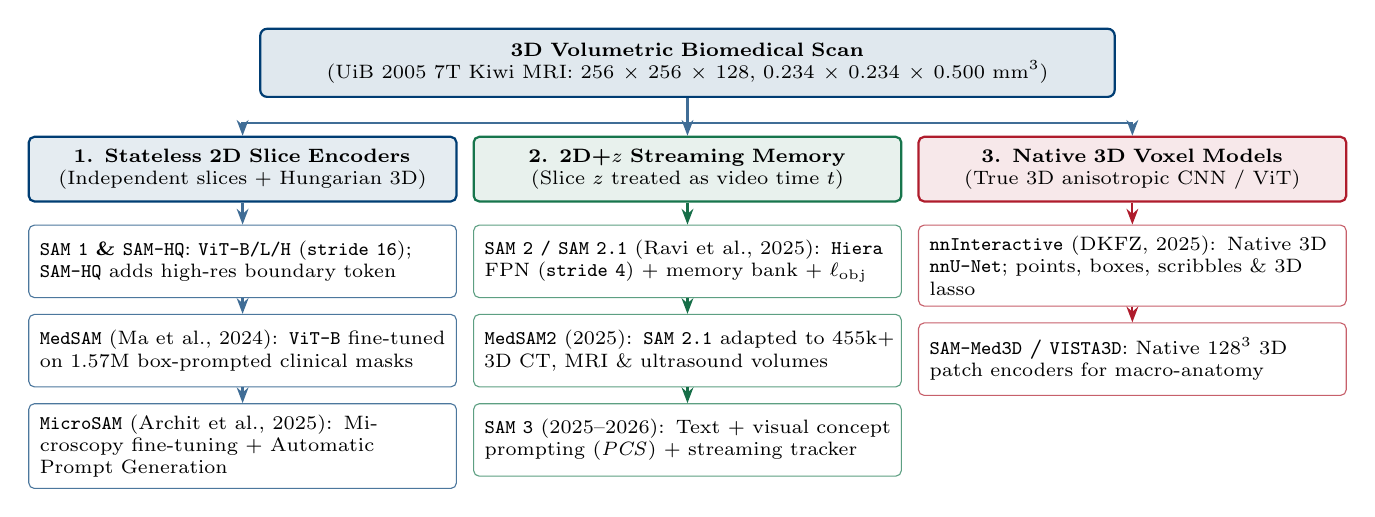
\begin{tikzpicture}[
    font=\scriptsize,
    root/.style={rectangle, rounded corners=2.5pt, draw=uibblue, fill=uibblue!12, thick, align=center, inner sep=5pt, text width=10.5cm},
    cat/.style={rectangle, rounded corners=2pt, draw=#1, fill=#1!10, thick, align=center, inner sep=4pt, text width=5.15cm, minimum height=0.82cm},
    leaf/.style={rectangle, rounded corners=2pt, draw=#1!70, fill=white, align=left, inner sep=4pt, text width=5.15cm, minimum height=0.92cm},
    arr/.style={-{Stealth[length=2mm,width=1.5mm]}, thick, draw=uibblue!75}
]
\node[root] (top) {\textbf{3D Volumetric Biomedical Scan}\\(UiB 2005 7T Kiwi MRI: $256 \times 256 \times 128$, $0.234 \times 0.234 \times 0.500\text{ mm}^3$)};

\node[cat=uibblue] (b1) at (-5.65cm, -1.35cm) {\textbf{1. Stateless 2D Slice Encoders}\\(Independent slices + Hungarian 3D)};
\node[cat=kiwigreen!85!black] (b2) at (0cm, -1.35cm) {\textbf{2. 2D+$z$ Streaming Memory}\\(Slice $z$ treated as video time $t$)};
\node[cat=uibred] (b3) at (5.65cm, -1.35cm) {\textbf{3. Native 3D Voxel Models}\\(True 3D anisotropic CNN / ViT)};

\draw[arr] (top.south) -- ++(0,-0.32) -| (b1.north);
\draw[arr] (top.south) -- (b2.north);
\draw[arr] (top.south) -- ++(0,-0.32) -| (b3.north);

% Column 1 leaves
\node[leaf=uibblue, below=0.28cm of b1] (l11) {\textbf{\texttt{SAM 1} \& \texttt{SAM-HQ}}: \texttt{ViT-B/L/H} (\texttt{stride 16}); \texttt{SAM-HQ} adds high-res boundary token};
\node[leaf=uibblue, below=0.20cm of l11] (l12) {\textbf{\texttt{MedSAM}} (Ma et al., 2024): \texttt{ViT-B} fine-tuned on 1.57M box-prompted clinical masks};
\node[leaf=uibblue, below=0.20cm of l12] (l13) {\textbf{\texttt{MicroSAM}} (Archit et al., 2025): Microscopy fine-tuning + Automatic Prompt Generation};

\draw[arr] (b1) -- (l11); \draw[arr] (l11) -- (l12); \draw[arr] (l12) -- (l13);

% Column 2 leaves
\node[leaf=kiwigreen!85!black, below=0.28cm of b2] (l21) {\textbf{\texttt{SAM 2 / SAM 2.1}} (Ravi et al., 2025): \texttt{Hiera} FPN (\texttt{stride 4}) + memory bank + $\ell_{\text{obj}}$};
\node[leaf=kiwigreen!85!black, below=0.20cm of l21] (l22) {\textbf{\texttt{MedSAM2}} (2025): \texttt{SAM 2.1} adapted to 455k+ 3D CT, MRI \& ultrasound volumes};
\node[leaf=kiwigreen!85!black, below=0.20cm of l22] (l23) {\textbf{\texttt{SAM 3}} (2025--2026): Text + visual concept prompting (\emph{PCS}) + streaming tracker};

\draw[arr, draw=kiwigreen!80!black] (b2) -- (l21); \draw[arr, draw=kiwigreen!80!black] (l21) -- (l22); \draw[arr, draw=kiwigreen!80!black] (l22) -- (l23);

% Column 3 leaves
\node[leaf=uibred, below=0.28cm of b3] (l31) {\textbf{\texttt{nnInteractive}} (DKFZ, 2025): Native 3D \texttt{nnU-Net}; points, boxes, scribbles \& 3D lasso};
\node[leaf=uibred, below=0.20cm of l31] (l32) {\textbf{\texttt{SAM-Med3D} / \texttt{VISTA3D}}: Native $128^3$ 3D patch encoders for macro-anatomy};

\draw[arr, draw=uibred] (b3) -- (l31); \draw[arr, draw=uibred] (l31) -- (l32);
\end{tikzpicture}
\caption{Taxonomy of 2024--2026 promptable segmentation foundation models by 3D volumetric strategy.}
\end{figure}

\begin{table}[H]
\centering
\scriptsize
\renewcommand{\arraystretch}{1.22}
\rowcolors{2}{white}{rowalt}
\begin{tabularx}{\textwidth}{L{2.0cm} L{2.7cm} L{2.3cm} L{2.3cm} L{2.6cm} Y}
\toprule
\rowcolor{uibblue!14}
\textbf{Model Family} & \textbf{HF / Package ID} & \textbf{Prompts} & \textbf{3D Strategy} & \textbf{Access \& Hardware} & \textbf{Behaviour on 7T Kiwi Seeds} \\
\midrule
\textbf{\texttt{SAM 2.1}} \newline (Meta, 2024--25) & \texttt{facebook/sam2.1-} \texttt{hiera-small} \newline (\texttt{transformers}) & Pos/neg points, boxes, masks & \textbf{Native slice memory} (\texttt{Sam2VideoModel}) + static 2D & \textbf{Ungated Apache-2.0} ($\sim 184\text{ MB}$); CUDA, Apple MPS, Colab, CPU & \textbf{Best primary choice:} Hiera \texttt{stride-4} FPN + Patch-Zoom resolves 5-px seeds (\texttt{2D IoU = 0.628}; 1-click 3D \texttt{PQ = 0.500}) \\
\textbf{\texttt{MedSAM}} \newline (Ma et al., 2024) & \texttt{wanglab/medsam-} \texttt{vit-base} \newline (\texttt{transformers}) & \textbf{Bounding boxes only} & 2D slice-by-slice + Hungarian IoU & \textbf{Ungated} ($\sim 375\text{ MB}$); CUDA, Apple MPS, Colab & \textbf{Key contrast:} Fails on 1-point (\texttt{IoU = 0.037}) \& full-slice boxes (\texttt{0.277}), but jumps to \textbf{\texttt{0.602}} when zoomed with tight boxes \\
\textbf{\texttt{SAM-HQ}} \newline (Ke et al., 2023) & \texttt{syscv-community/} \texttt{sam-hq-vit-base} & Points \& boxes & 2D slice-by-slice & \textbf{Ungated}; native in \texttt{transformers} & Early ViT features + \texttt{HQ-Token} sharpen thin boundaries over \texttt{SAM-1} \\
\textbf{\texttt{MedSAM2}} \newline (Wang Lab, 2025) & \texttt{wanglab/MedSAM2} \newline (GitHub clone) & Boxes \& clicks on key MRI slice & \textbf{3D slice memory} trained on 455k+ 3D scans & Ungated weights; custom repo outside \texttt{uv.lock} & Strong clinical lesion tracker; behaves similarly to physically gated \texttt{Sam2VideoModel} \\
\textbf{\texttt{MicroSAM}} \newline (Archit et al., 2025) & \texttt{micro\_sam} \newline (\texttt{vit\_b\_lm}) & Points, boxes, + Auto-Prompt (\texttt{APG}) & 2D + 3D microscopy tracking (Napari) & Open source; heavy \texttt{elf}/\texttt{vigra} deps outside root \texttt{uv} & Closest domain pretraining for packed cells/vesicles; ideal for a Block 2 Individual Project \\
\textbf{\texttt{nnInteractive}} \newline (DKFZ, 2025) & \texttt{MIC-DKFZ/} \texttt{nnInteractive} & 3D points, boxes, scribbles, lasso & \textbf{True native 3D anisotropic CNN} & \textbf{NVIDIA CUDA required} (Napari / MITK / Slicer) & Gold-standard interactive 3D clinical annotator on Linux/CUDA workstations \\
\textbf{\texttt{SAM 3}} \newline (Meta, 2025--26) & \texttt{facebook/sam3} \newline (\texttt{transformers}) & \textbf{Text phrases} + points/boxes & Unified detector + streaming tracker & \textbf{Gated HF repo} (license form + \texttt{HF\_TOKEN}) & Adds text-prompted concept segmentation (\emph{PCS}), though gating adds classroom friction \\
\bottomrule
\end{tabularx}
\caption{Practical selection matrix for BMED365 (\texttt{bmed365-2027} local \texttt{uv} environment and free Google Colab).}
\end{table}

% =====================================================================
% SECTION 4: MATHEMATICAL & BIOPHYSICAL FAILURE MODES
% =====================================================================
\section{Mathematical \& Biophysical Analysis of the Four Kiwi Failure Modes}

\subsection{Trap 1 --- The ViT Token-Stride Bottleneck \& Patch-Zoom Remedy}
\label{sec:trap1}

Suppose a 2D MRI slice of matrix size $N_{\text{slice}} \times N_{\text{slice}}$ ($256 \times 256$) and in-plane pixel spacing $\Delta x = 0.2344\text{ mm}$ is resized to $N_{\text{enc}} \times N_{\text{enc}}$ ($1024 \times 1024$) and tokenized with patch stride $s_{\text{enc}} = 16$ (\texttt{ViT-B/16}), yielding a $64 \times 64$ token grid ($N_{\text{grid}} = N_{\text{enc}} / s_{\text{enc}} = 64$). The physical width of \textbf{one encoder feature token} in the specimen is:
\[
    \Delta_{\text{tok}} = \frac{N_{\text{slice}}}{N_{\text{grid}}}\,\Delta x = \frac{256}{64} \times 0.2344\text{ mm} = 0.938\text{ mm}.
\]
Compare $\Delta_{\text{tok}} = 0.938\text{ mm}$ against a mature \texttt{'Hayward'} kiwifruit seed:
\begin{itemize}
    \item Minor equatorial diameter $d_{\min} \approx 1.0\text{--}1.3\text{ mm} \implies$ \textbf{only $1.1\text{--}1.4$ ViT tokens wide!}
    \item By spatial Nyquist sampling, resolving seed curvature and the thin bright mucilage cleft ($\sim 0.25\text{--}0.45\text{ mm}$) between touching seeds requires $\Delta_{\text{tok}} \lesssim 0.20\text{ mm}$ ($\ge 5\text{--}6$ tokens across each seed).
\end{itemize}
\textbf{Two-Part Architectural Remedy:}
\begin{enumerate}
    \item \textbf{ROI / Tile Patch-Zoom:} Cropping an $80 \times 40$ sector (or tiling overlapping $64 \times 64$ patches across $256 \times 256$) shrinks the physical token footprint $3.2\times$:
    \[
        \Delta_{\text{tok}}^{\text{zoom}} = \frac{80}{64} \times 0.2344\text{ mm} = 0.293\text{ mm}.
    \]
    \item \textbf{Multi-Scale Hiera FPN Skip Connections (\texttt{SAM 2.1}):} Unlike plain \texttt{ViT-B/16} (\texttt{SAM-1} / \texttt{MedSAM}), \texttt{SAM 2.1}'s hierarchical \textbf{Hiera} backbone injects \textbf{\texttt{stride-4} ($256 \times 256$ feature grid)} and \textbf{\texttt{stride-8} ($128 \times 128$)} skip features directly into the mask decoder's transposed convolutions --- pushing effective spatial resolution on an $80 \times 80$ crop down to $\Delta_{\text{fpn}} \approx 0.073\text{ mm}$ (sub-pixel relative to the $0.234\text{ mm}$ 7T acquisition!).
\end{enumerate}

\subsection{Trap 2 --- Prompt Modality Mismatch (\texttt{MedSAM} vs.\ \texttt{SAM 2.1}) \& Scale Ambiguity}

\begin{itemize}
    \item \textbf{Why \texttt{MedSAM} Collapses on Point Clicks:} Ma et al.\ (2024) trained \texttt{MedSAM} on $1.57\text{M}$ medical image--mask pairs using \textbf{bounding-box prompts} (matching clinical RECIST calipers) while omitting single-point disambiguation training. Passing a 1-point click to \texttt{wanglab/medsam-vit-base} produces diffuse masks spilling across half the pericarp (\texttt{Mean 2D Seed IoU = 0.037} full-slice; \texttt{0.107} even zoomed!). Supplying a \textbf{tight physical box ($\pm 0.8\text{ px}$)} on a \textbf{zoomed $80 \times 40$ ROI} lifts \texttt{MedSAM} \textbf{$16\times$ to \texttt{IoU = 0.602} (\texttt{2D Dice = 0.748})}.
    \item \textbf{Resolving Single-Point Scale Ambiguity in \texttt{SAM 2.1}:} With \texttt{multimask\_output=True} on a single click $(x_p, y_p)$, \texttt{SAM 2.1} outputs three nested hypotheses ordered $(M_0, M_1, M_2)$: \textbf{finest sub-part ($M_0$: single seed)} $\to$ \textbf{part ($M_1$: radial locule)} $\to$ \textbf{whole organ ($M_2$: whole fruit)}. Ranking naively by $\arg\max_m \widehat{\text{IoU}}_m$ in unprompted grids overwhelmingly picks macroscopic \emph{Stuff} ($M_1, M_2$, where outer peel borders score $\widehat{\text{IoU}} > 0.95$; \textbf{52 Stuff masks vs.\ 4 seed masks} on an $8\times 8$ grid!). Selecting \textbf{sub-part head $m = 0$} --- or pairing the click with a standardized physical box $[x_p \pm r_{\text{box}}, y_p \pm r_{\text{box}}]$ ($r_{\text{box}} \approx 0.75\text{ mm} = 3.2\text{ px}$, \texttt{multimask\_output=False}) --- eliminates whole-organ bleed completely.
\end{itemize}

\subsection{Trap 3 --- Anisotropic 2D-to-3D Slice Memory Drift (\texttt{Sam2VideoModel})}

In \texttt{Sam2VideoModel}, we treat the 3D MRI sub-volume $I(x, y, z)$ ($z \in \{0, \dots, Z-1\}$) as a video stream where axial slice $z$ acts as frame $t$, propagating bidirectionally ($z_0 \to z_0 + 1 \dots$ and $z_0 \to z_0 - 1 \dots$) from a single equatorial click at $z_0$.

\textbf{Why Unbounded Propagation ($\Delta z_{\max} = \infty$) Fails:} A kiwifruit seed of length $L_z \approx 2.0\text{--}2.4\text{ mm}$ spans only $L_z / \Delta z \approx 4\text{--}5$ slices ($\lvert z - z_0 \rvert \le 2$). Because up to 40--50 seeds sit inside one radial chamber, another seed frequently appears at nearly the same $(x, y)$ coordinate $2\text{--}3$ slices above or below. Unbounded memory attention locks onto the next seed in the chamber, causing \textbf{vertical $z$-axis instance merges} (\texttt{10--13} merged clumps on the 52-seed wedge, dropping \texttt{PQ} to \texttt{0.297--0.323}). Truncating propagation with \textbf{three domain invariants} solves $z$-drift:
\begin{enumerate}
    \item \textbf{Physical $z$-horizon:} $\lvert z - z_0 \rvert \le \Delta z_{\max} = \lceil 1.1\text{ mm} / 0.50\text{ mm} \rceil = 2$ slices (max $2.5\text{ mm}$ span).
    \item \textbf{Learned occlusion stop:} Require \texttt{object\_score\_logits} $> 0$ (halting when \texttt{SAM 2.1} detects the seed pole has ended).
    \item \textbf{Lateral \& $T_2$-contrast gate:} Require $\lVert(x,y) - (x_0,y_0)\rVert_2 \le 1.2\text{ mm}$ and $I(x,y,z) < 0.52\,E_{\text{gel}}(x,y,z)$.
\end{enumerate}

\subsection{Trap 4 --- Neurosymbolic Prompt Generation (\emph{Physics Proposals + Neural Decoding})}

\begin{figure}[ht!]
\centering
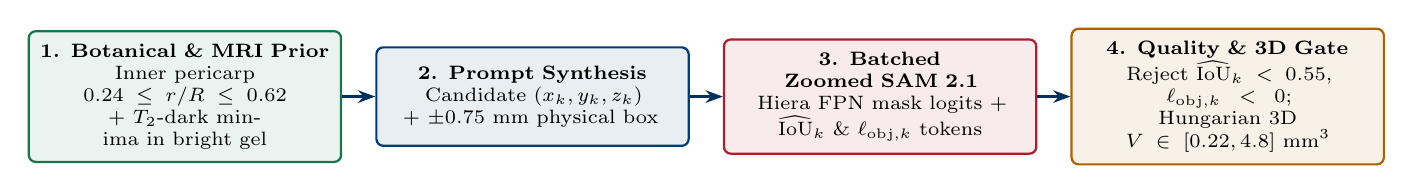
\begin{tikzpicture}[
    font=\scriptsize,
    stage/.style={rectangle, rounded corners=2.5pt, draw=#1, fill=#1!9, thick, align=center, inner sep=4.5pt, text width=3.65cm, minimum height=1.25cm},
    arr/.style={-{Stealth[length=2.2mm,width=1.6mm]}, thick, draw=uibblue!80!black}
]
\node[stage=kiwigreen!85!black] (s1) {\textbf{1. Botanical \& MRI Prior}\\Inner pericarp $0.24 \le r/R \le 0.62$\\+ $T_2$-dark minima in bright gel};
\node[stage=uibblue, right=0.42cm of s1] (s2) {\textbf{2. Prompt Synthesis}\\Candidate $(x_k, y_k, z_k)$\\+ $\pm 0.75\text{ mm}$ physical box};
\node[stage=uibred, right=0.42cm of s2] (s3) {\textbf{3. Batched Zoomed SAM 2.1}\\Hiera FPN mask logits +\\$\widehat{\text{IoU}}_k$ \& $\ell_{\text{obj},k}$ tokens};
\node[stage=amberwarn!90!black, right=0.42cm of s3] (s4) {\textbf{4. Quality \& 3D Gate}\\Reject $\widehat{\text{IoU}}_k < 0.55$, $\ell_{\text{obj},k} < 0$;\\Hungarian 3D $V \in [0.22, 4.8]\text{ mm}^3$};

\draw[arr] (s1) -- (s2);
\draw[arr] (s2) -- (s3);
\draw[arr] (s3) -- (s4);
\end{tikzpicture}
\caption{Zero-training neurosymbolic 3D seed segmentation pipeline combining botanical priors with \texttt{SAM 2.1} confidence gating.}
\end{figure}

\begin{infobox}[Why the Botanical Radial Zone ($0.24 \le r/R \le 0.62$) Is Essential]
As illustrated in the companion \href{https://github.com/arvidl/BMED365-2027/blob/main/Lab5-Comp-Mod/Kiwi-challenge/notebooks/00a-kiwi-anatomical-and-physiological-atlas.ipynb}{\textbf{Multi-Scale Anatomical \& Histological Atlas (\texttt{Lab 5 / 00a})}}, \emph{Actinidia} seeds develop \textbf{exclusively} on axile placentae inside the inner pericarp locules ($0.24 \le r/R \le 0.62$). Both the central fibrous \emph{columella} ($r/R < 0.24$) and the dimorphic outer cortex parenchyma ($r/R > 0.62$) contain dark $T_2$ pockets (vascular bundles, starch-rich cells, Rician speckle) that mimic seeds locally. Constraining candidate proposals to $0.24 \le r/R \le 0.62$ cuts 3D prompt false positives from 80 down to \textbf{52 (matching $\text{GT} = 52$)} --- directly analogous to \textbf{brain extraction and white/grey-matter atlas masking} before cerebral microbleed detection!
\end{infobox}

% =====================================================================
% SECTION 5: EMPIRICAL BENCHMARK ON APPLE M4 MAX (MPS)
% =====================================================================
\section{Empirical Benchmark on the 2005 UiB 7T Kiwi MRI}

All benchmarks below were executed on the \textbf{held-out 3D test sub-volume ($80 \times 40 \times 16$ voxels = $18.75 \times 9.38 \times 8.00\text{ mm}^3$, 52 unseen 3D ground-truth seeds)} defined in Notebook~\texttt{04} and reproduced in \href{https://github.com/arvidl/BMED365-2027/blob/main/Lab4-Comp-Imag/Kiwi-challenge/notebooks/05-kiwi-promptable-foundation-models.ipynb}{\textbf{Notebook~\texttt{05}}}, running on an Apple MacBook Pro M4 Max (\texttt{mps} backend, \texttt{float32}, \texttt{transformers 4.57.6}).

\begin{figure}[ht!]
\centering
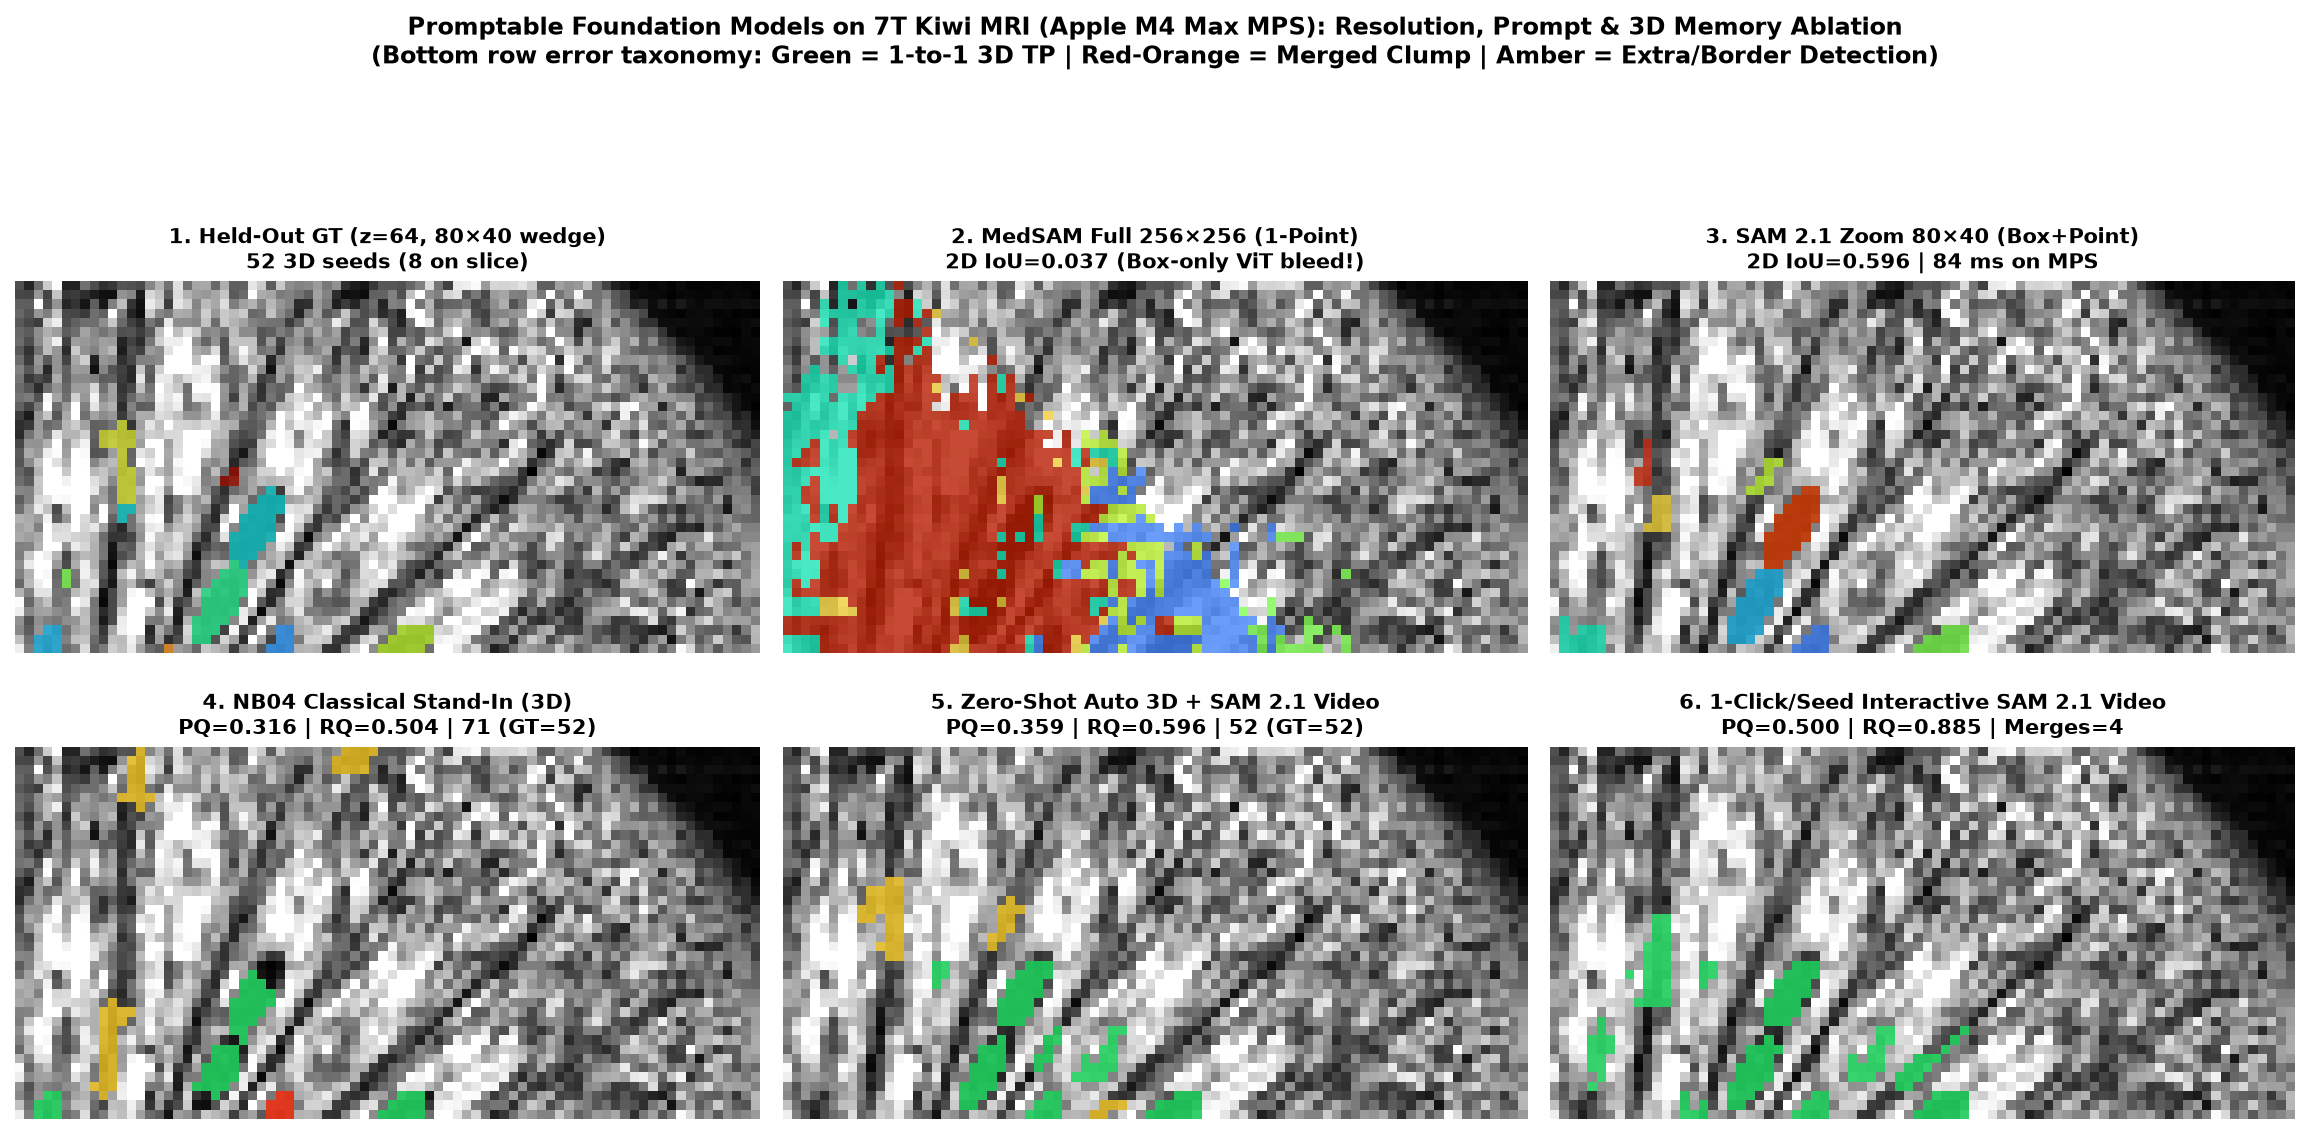
\includegraphics[width=\textwidth]{../assets/kiwi_foundation_model_benchmark.png}
\caption{Six-panel visual comparison on equatorial slice $z = 64$ of the held-out $80 \times 40 \times 16$ test wedge. \textbf{Top row:} Ground truth (8 visible seeds), \texttt{MedSAM} full-slice 1-point failure (\texttt{IoU = 0.037}), and Patch-Zoomed \texttt{SAM 2.1} box+point recovery (\texttt{IoU = 0.596}, $84\text{ ms}$). \textbf{Bottom row (3D error taxonomy: Green = 1-to-1 TP, Red-Orange = Merged Clump, Amber = Extra/Border):} Notebook~\texttt{04} classical stand-in (\texttt{PQ = 0.316}), zero-shot neurosymbolic \texttt{SAM 2.1} video (\texttt{PQ = 0.359}, exact 52/52 count), and 1-click/seed interactive \texttt{SAM 2.1} video (\texttt{PQ = 0.500}, \texttt{RQ = 0.885}).}
\end{figure}

\begin{table}[ht!]
\centering
\scriptsize
\renewcommand{\arraystretch}{1.18}
\rowcolors{2}{white}{rowalt}
\begin{tabularx}{\textwidth}{L{2.7cm} L{1.75cm} L{2.15cm} C{1.45cm} C{1.45cm} R{1.35cm} Y}
\toprule
\rowcolor{uibblue!14}
\textbf{Model Checkpoint} & \textbf{Input Scope} & \textbf{Prompt Modality} & \textbf{Mean 2D Seed IoU} & \textbf{2D Sem.\ Dice} & \textbf{M4 Max \texttt{mps}} & \textbf{Key Diagnostic Lesson} \\
\midrule
\textbf{\texttt{MedSAM}} (\texttt{vit-base}) & Full $256^2$ & \texttt{1-Point} & 0.037 & 0.165 & $411\text{ ms}$ & \textbf{Collapse:} box-only decoder spills across pericarp \\
\textbf{\texttt{MedSAM}} (\texttt{vit-base}) & Full $256^2$ & \texttt{Tight Box} ($\pm 0.8\text{ px}$) & 0.277 & 0.491 & $238\text{ ms}$ & \textbf{Token blur:} 1 \texttt{ViT-B/16} token $= 0.94\text{ mm}$ ($\sim 1$ seed) \\
\textbf{\texttt{MedSAM}} (\texttt{vit-base}) & \textbf{Zoom $80\times 40$} & \texttt{1-Point} & 0.107 & 0.237 & $240\text{ ms}$ & Zooming alone cannot fix untrained point prompts \\
\textbf{\texttt{MedSAM}} (\texttt{vit-base}) & \textbf{Zoom $80\times 40$} & \textbf{\texttt{Tight Box}} & \textbf{0.602} & \textbf{0.748} & $234\text{ ms}$ & \textbf{$2.17\times$ IoU jump!} Matches box-prompted training \\
\textbf{\texttt{SAM 2.1}} (\texttt{hiera-small}) & Full $256^2$ & \texttt{1-Point} ($m=0$) & 0.377 & 0.235 & $124\text{ ms}$ & $10\times$ above \texttt{MedSAM} 1-point, but full-FOV blurs edges \\
\textbf{\texttt{SAM 2.1}} (\texttt{hiera-small}) & Full $256^2$ & \texttt{Tight Box} ($\pm 0.8\text{ px}$) & 0.570 & 0.779 & $89\text{ ms}$ & Hiera \texttt{stride-4} FPN preserves seeds even at full FOV \\
\textbf{\texttt{SAM 2.1}} (\texttt{hiera-small}) & \textbf{Zoom $80\times 40$} & \texttt{1-Point} ($m=0$) & 0.520 & 0.603 & \textbf{$82\text{ ms}$} & Fast single-click seed delineation without boxes \\
\textbf{\texttt{SAM 2.1}} (\texttt{hiera-small}) & \textbf{Zoom $80\times 40$} & \textbf{\texttt{Tight Box}} & \textbf{0.628} & 0.694 & \textbf{$82\text{ ms}$} & Highest per-seed 2D IoU ($82\text{ ms}$ batched for 8 seeds) \\
\textbf{\texttt{SAM 2.1}} (\texttt{hiera-small}) & \textbf{Zoom $80\times 40$} & \textbf{\texttt{Box + Point}} & 0.596 & \textbf{0.795} & \textbf{$84\text{ ms}$} & Best 2D Dice (\emph{inverted contrast gives 0.801: polarity-invariant}) \\
\bottomrule
\end{tabularx}
\caption{2D Slice $z = 64$ resolution and prompt modality ablation (oracle prompts on 8 visible seeds).}
\end{table}

\begin{table}[ht!]
\centering
\scriptsize
\renewcommand{\arraystretch}{1.2}
\rowcolors{2}{white}{rowalt}
\begin{tabularx}{\textwidth}{Y C{1.15cm} C{1.15cm} C{0.95cm} C{0.90cm} C{0.85cm} C{0.80cm} C{0.85cm} C{0.95cm} C{0.95cm} R{1.15cm}}
\toprule
\rowcolor{uibblue!14}
\textbf{3D Segmentation Paradigm} & \textbf{Kiwi Train} & \textbf{Test Clicks} & \textbf{Pred ($\text{GT}\!=\!52$)} & \textbf{Sem.\ Dice} & \textbf{Merge} & \textbf{Split} & \textbf{SQ} & \textbf{RQ ($F_1$)} & \textbf{PQ} & \textbf{Time (\texttt{mps})} \\
\midrule
1. Classical 4-Class K-Means + 3D CC (\emph{NB 04}) & 0 & 0 & 17 & 0.487 & 10 & 0 & 0.506 & 0.174 & 0.088 & $<0.2\text{ s}$ \\
2. Supervised 3D Semantic U-Net + CC (\emph{NB 04}) & 46 seeds & 0 & 36 & 0.690 & 11 & 0 & 0.564 & 0.432 & 0.244 & $\sim 5.5\text{ s}$ \\
3. Classical Heuristic Stand-In (\emph{NB 04 Step 4}) & 0 & 0 & 71 & 0.529 & 3 & 0 & 0.627 & 0.504 & 0.316 & $<0.2\text{ s}$ \\
4. Zero-Shot Auto 3D + \texttt{SAM 2.1} Video (no prior) & 0 & 0 & 80 & 0.459 & 2 & 0 & 0.601 & 0.470 & 0.282 & $26.0\text{ s}$ \\
\textbf{5. Zero-Shot Auto 3D + Prior + \texttt{SAM 2.1} Video} & \textbf{0} & \textbf{0} & \textbf{52} & 0.579 & \textbf{2} & \textbf{0} & 0.601 & 0.596 & \textbf{0.359} & $21.1\text{ s}$ \\
\textbf{6. Zero-Shot Batched 2D \texttt{SAM 2.1} + $\widehat{\text{IoU}}$ Gate} & \textbf{0} & \textbf{0} & 43 & 0.617 & 3 & \textbf{0} & 0.618 & \textbf{0.632} & \textbf{0.390} & \textbf{$1.4\text{--}2.2\text{ s}$} \\
7. Supervised 3D Multi-Task U-Net (\emph{NB 04}) & 46 seeds & 0 & 54 & 0.651 & \textbf{2} & 1 & \textbf{0.670} & 0.604 & \textbf{0.405} & $\sim 5.5\text{ s}$ \\
8. Interactive 1-Click/Seed + \texttt{SAM 2.1} (unbounded $z$) & 0 & 52 clicks & 52 & 0.584 & 10 & 8 & 0.542 & 0.596 & 0.323 & $146.2\text{ s}$ \\
\textbf{9. Interactive 1-Click/Seed + \texttt{SAM 2.1} ($\lvert\Delta z\rvert \le 2$)} & \textbf{0} & \textbf{52 clicks} & \textbf{52} & \textbf{0.761} & 4 & 4 & 0.565 & \textbf{0.885} & \textbf{0.500} & \textbf{$23.0\text{ s}$} \\
\bottomrule
\end{tabularx}
\caption{Full 3D benchmark on the held-out $80 \times 40 \times 16$ test wedge ($\text{GT} = 52$ unseen 3D seeds, Hungarian matching at $\text{IoU} \ge 0.25$).}
\end{table}

\subsection{Key Empirical Takeaways}

\begin{enumerate}
    \item \textbf{Zero-Training Neurosymbolic \texttt{SAM 2.1} Nearly Matches Supervised 3D Deep Learning (\texttt{PQ = 0.390} vs.\ \texttt{0.405}):} Combining inner-pericarp radial gating ($0.24 \le r/R \le 0.62$), batched zoomed \texttt{SAM 2.1} decoding, $\widehat{\text{IoU}} \ge 0.55$ confidence filtering, and Hungarian 3D slice linking runs in \textbf{$1.4\text{--}2.2\text{ s}$} with \textbf{zero kiwi training labels}, beating the supervised 3D Multi-Task U-Net on 3D Instance $F_1$ (\texttt{RQ = 0.632} vs.\ \texttt{0.604}). Meanwhile, 3D peak proposals + \texttt{Sam2VideoModel} recover the \textbf{exact 52/52 seed count} (\texttt{PQ = 0.359}, 0 split errors).
    \item \textbf{Interactive ``1 Click = 1 3D Seed'' Curation (\texttt{PQ = 0.500}, \texttt{RQ = 0.885}):} Clicking once at a seed's equatorial slice $z_0$ and propagating $\lvert\Delta z\rvert \le 2$ slices achieves \textbf{88.5\% 3D Instance $F_1$} at $0.44\text{ s/seed}$, cutting manual slice-by-slice brush strokes in Notebook~\texttt{03b} by $\sim 75\text{--}80\%$.
    \item \textbf{Unbounded Video Memory Degrades Anisotropic 3D MRI:} Comparing Rows~8 and~9 proves that unbounded $z$-tracking drops \texttt{PQ} from \texttt{0.500} to \texttt{0.323} ($2.5\times$ more merges, $6.4\times$ slower) due to vertical seed-to-seed jumping across $0.50\text{ mm}$ slice steps.
    \item \textbf{Whole-Organ Generalization ($256 \times 256 \times 128$) Without Polar OOD Explosion:} In Notebook~\texttt{04}, sliding an equatorial-trained 3D U-Net across polar slices ($z < 40, z > 88$) over-predicted \texttt{3,328} raw blobs on oblique polar vascular bundles. In Notebook~\texttt{05}, slice-cropped batched \texttt{SAM 2.1} + $\widehat{\text{IoU}} \ge 0.55$ across all 128 slices finishes in \textbf{$24.0\text{ s}$} on \texttt{mps}, tapering smoothly to zero at both poles with \textbf{1,532 raw 3D seeds}, Micro-GT ratio-calibrated \textbf{$\widehat{N}_{\text{cal}} = 1{,}668$ seeds} ($P = 0.667, R = 0.612$), mean seed volume \textbf{$1.51\text{ mm}^3$} (Micro-GT median: $1.524\text{ mm}^3$), and whole-berry \textbf{``lesion load'' $= 2.68\%$} ($85.97\text{ cm}^3$ fruit).
\end{enumerate}

% =====================================================================
% SECTION 6: REPRODUCIBLE CODE RECIPES
% =====================================================================
\section{Reproducible Code Recipes (\texttt{bmed365-2027} Local \texttt{uv} \& Google Colab)}

\begin{warningbox}[Apple Silicon (\texttt{MPS}) \texttt{float64} Tensor Gotcha]
Hugging Face's \texttt{SamProcessor} and \texttt{Sam2Processor} convert Python \texttt{float} coordinates in \texttt{input\_points} / \texttt{input\_boxes} into \texttt{torch.float64} tensors by default. Calling \texttt{inputs.to("mps")} directly raises \texttt{TypeError: Cannot convert a MPS Tensor to float64 dtype}. Always downcast floating-point prompt tensors to \texttt{torch.float32} via \texttt{to\_device\_fp32(...)} below so identical code runs on \textbf{macOS M1--M5 (\texttt{mps})}, \textbf{Linux (\texttt{cuda})}, \textbf{Google Colab (\texttt{T4})}, and \textbf{CPU}.
\end{warningbox}

\subsection{Batched 2D Patch-Zoom \texttt{SAM 2.1} Decoding with Confidence Tokens}

\begin{lstlisting}[style=pybmed]
import numpy as np
import torch
from PIL import Image
from transformers import Sam2Model, Sam2Processor

device = torch.device(
    "cuda" if torch.cuda.is_available()
    else ("mps" if hasattr(torch.backends, "mps") and torch.backends.mps.is_available() else "cpu")
)

def to_device_fp32(batch: dict, dev: torch.device) -> dict:
    """Safe transfer for CUDA, Apple Silicon MPS (no float64!), and CPU."""
    out = {}
    for k, v in batch.items():
        if isinstance(v, torch.Tensor):
            if v.is_floating_point() and v.dtype == torch.float64:
                v = v.to(dtype=torch.float32)
            out[k] = v if k in ("original_sizes", "reshaped_input_sizes") else v.to(dev)
        else:
            out[k] = v
    return out

def slice_xy_to_pil(sl_xy: np.ndarray) -> Image.Image:
    """Transpose (SX, SY) NIfTI slice to (H=SY, W=SX) RGB PIL image so voxel (ix, iy) == prompt [x=ix, y=iy]."""
    u8 = (np.clip(sl_xy, 0.0, 1.0).T * 255.0).round().astype(np.uint8)
    return Image.fromarray(np.stack([u8, u8, u8], axis=-1))

sam2_id = "facebook/sam2.1-hiera-small"  # Ungated Apache-2.0 (~184 MB)
processor = Sam2Processor.from_pretrained(sam2_id)
model = Sam2Model.from_pretrained(sam2_id).to(device).eval()

def decode_zoomed_slice_seeds(sl_xy: np.ndarray, seed_xy_pts: list[tuple[float, float]], r_box: float = 3.2):
    pil_img = slice_xy_to_pil(sl_xy)
    pts = [[[x, y]] for x, y in seed_xy_pts]
    lbls = [[1] for _ in seed_xy_pts]
    boxes = [[x - r_box, y - r_box, x + r_box, y + r_box] for x, y in seed_xy_pts]

    raw_in = processor(images=pil_img, input_points=[pts], input_labels=[lbls], input_boxes=[boxes], return_tensors="pt")
    model_in = to_device_fp32(raw_in, device)
    with torch.no_grad():
        out = model(
            pixel_values=model_in["pixel_values"], input_points=model_in["input_points"],
            input_labels=model_in["input_labels"], input_boxes=model_in["input_boxes"], multimask_output=False,
        )
    mask_logits = processor.post_process_masks(out.pred_masks.cpu(), raw_in["original_sizes"], binarize=False)[0]
    iou_scores = out.iou_scores.cpu()[0, :, 0].numpy()
    obj_logits = out.object_score_logits.cpu()[0, :, 0].numpy()
    return mask_logits[:, 0].numpy().transpose(0, 2, 1), iou_scores, obj_logits
\end{lstlisting}

\subsection{Bidirectional 3D Slice Memory Propagation (\texttt{Sam2VideoModel})}

\begin{lstlisting}[style=pybmed]
from transformers import Sam2VideoModel, Sam2VideoProcessor

vid_proc = Sam2VideoProcessor.from_pretrained("facebook/sam2.1-hiera-small")
vid_model = Sam2VideoModel.from_pretrained("facebook/sam2.1-hiera-small").to(device).eval()

def propagate_single_3d_seed(sub_vol: np.ndarray, x0: float, y0: float, z0: int, r_box: float = 3.2, max_dz: int = 2):
    """1-Click 3D seed segmentation: prompt at (x0, y0, z0) and propagate +-max_dz slices."""
    frames = [slice_xy_to_pil(sub_vol[:, :, z]) for z in range(sub_vol.shape[2])]
    sx, sy, sz = sub_vol.shape
    session = vid_proc.init_video_session(
        video=frames, inference_device=device, processing_device="cpu", video_storage_device=device, dtype=torch.float32
    )
    vid_proc.add_inputs_to_inference_session(
        inference_session=session, frame_idx=z0, obj_ids=[1],
        input_points=torch.tensor([[[[x0, y0]]]], dtype=torch.float32),
        input_labels=torch.tensor([[[1]]], dtype=torch.int32),
        input_boxes=torch.tensor([[[x0 - r_box, y0 - r_box, x0 + r_box, y0 + r_box]]], dtype=torch.float32),
    )
    mask_3d = np.zeros((sx, sy, sz), dtype=bool)
    with torch.no_grad():
        _ = vid_model(inference_session=session, frame_idx=z0)
        for rev in (False, True):
            for step_out in vid_model.propagate_in_video_iterator(
                inference_session=session, start_frame_idx=z0, max_frame_num_to_track=max_dz, reverse=rev
            ):
                z_cur = int(step_out.frame_idx)
                if abs(z_cur - z0) <= max_dz and float(step_out.object_score_logits.cpu().view(-1)[0]) > 0.0:
                    logits_yx = vid_proc.post_process_masks(
                        [step_out.pred_masks.cpu()], original_sizes=[(sy, sx)], binarize=False
                    )[0][0, 0].numpy()
                    mask_3d[:, :, z_cur] |= logits_yx.T > 0.0
    return mask_3d
\end{lstlisting}

% =====================================================================
% SECTION 7: SELF-CHECK QUESTIONS, BLOCK 2 PROJECTS & REFERENCES
% =====================================================================
\section{Self-Check Questions \& Block 2 Individual Project Ideas}

\begin{qabox}[Check Your Understanding Q1: Disentangling Resolution from Prompt Modality]
\textbf{Question:} Why did \texttt{MedSAM} (\texttt{wanglab/medsam-vit-base}) jump from \texttt{Mean 2D Seed IoU = 0.277} on the full $256 \times 256$ slice to \texttt{0.602} on the $80 \times 40$ ROI crop when given tight bounding boxes, yet remain stuck at \texttt{0.107} when given 1-point prompts on the exact same $80 \times 40$ crop?\\[3pt]
\textbf{Answer:} Two orthogonal mechanisms are at work: (1)~\textbf{Encoder spatial resolution (solved by Patch-Zoom):} \texttt{MedSAM} uses a plain \texttt{ViT-B/16} encoder without FPN skip connections ($64\times 64$ grid), so cropping from $256$ to $80\text{ px}$ shrinks each token from $0.94\text{ mm}$ to $0.29\text{ mm}$ ($\sim 4$ tokens across a seed), resolving contours under box prompts. (2)~\textbf{Decoder prompt conditioning (NOT solved by Patch-Zoom):} \texttt{MedSAM} was fine-tuned exclusively with bounding-box corner tokens (\texttt{labels 2, 3}); without box constraints, its mask decoder spills across surrounding tissue regardless of zoom factor.
\end{qabox}

\begin{qabox}[Check Your Understanding Q2: Anisotropic Slice Memory in Clinical Neuroimaging]
\textbf{Question:} Suppose you apply \texttt{Sam2VideoModel} to track \textbf{cerebral microbleeds (\texttt{CMBs})} vs.\ \textbf{perivascular spaces (\texttt{PVS})} across a clinical 3D \texttt{SWI} / $T_2$ brain MRI ($0.5 \times 0.5 \times 2.0\text{ mm}^3$ voxels). What happens if you leave \texttt{max\_frame\_num\_to\_track=None} (unbounded), and how should $\Delta z_{\max}$ be set from anatomy?\\[3pt]
\textbf{Answer:} At $2.0\text{ mm}$ slice thickness, a spherical cerebral microbleed ($1\text{--}3\text{ mm}$) spans only \textbf{1--2 slices} ($\Delta z_{\max} = 1$). Leaving tracking unbounded lets video memory jump onto dark cortical veins or basal ganglia iron across dozens of slices, turning a focal microbleed into a spurious vessel track. Conversely, tubular perivascular spaces run continuously over $10\text{--}15\text{ mm}$ ($\Delta z_{\max} \approx 5\text{--}7$), showing why physical morphology must govern memory horizon.
\end{qabox}

\subsection{Ideas for Block 2 Individual Projects (BMED365)}
\begin{enumerate}
    \item \textbf{Overlapping $64 \times 64$ Sliding-Tile \texttt{SAM 2.1} Whole-Berry Census:} Tile high-zoom $64 \times 64$ windows across the inner-pericarp ring of all 128 slices, fuse overlapping masks via 3D non-maximum suppression + $\widehat{\text{IoU}}$ calibration, and audit on Notebook~\texttt{03}'s \textbf{4-Panel Semi-Verifiability Dashboard}.
    \item \textbf{Interactive \texttt{SAM 2.1}-Assisted Silver-to-Gold GT Curation:} Add a \emph{``1-Click \texttt{SAM 2.1} 3D Seed''} mode to Notebook~\texttt{03b}'s \texttt{ipywidgets} delineator and quantify annotation speedup and multi-rater \texttt{STAPLE} agreement (\texttt{PQ} \& \texttt{DSC}) vs.\ manual voxel painting.
    \item \textbf{\texttt{Sim-to-Real} Decoder Fine-Tuning on the Lab 5 Bloch-MRI Digital Twin:} Freeze \texttt{SAM 2.1}'s Hiera encoder and fine-tune only its $\sim 4\text{M}$-parameter mask decoder on synthetic 7T scans with exact ground truth from \href{https://github.com/arvidl/BMED365-2027/blob/main/Lab5-Comp-Mod/Kiwi-challenge/notebooks/02-kiwi-digital-twin-and-inverse-problems.ipynb}{\texttt{Lab 5 / NB 02}}, testing zero-annotation transfer to the real 2005 UiB 7T scan.
    \item \textbf{Head-to-Head Benchmark Against \texttt{MicroSAM} or \texttt{nnInteractive}:} On a Linux CUDA workstation, compare \texttt{SAM 2.1} slice-memory propagation against \texttt{MicroSAM}'s Automatic Prompt Generator (\texttt{vit\_b\_lm}) or DKFZ's native 3D \texttt{nnInteractive}.
\end{enumerate}

\section*{Key References}
\addcontentsline{toc}{section}{Key References}
\small
\begin{enumerate}[label={[\arabic*]}]
    \item Kirillov A et al. \emph{Segment Anything.} \textbf{ICCV} (2023). \href{https://arxiv.org/abs/2304.02643}{arXiv:2304.02643}
    \item Ma J et al. \emph{Segment anything in medical images (\texttt{MedSAM}).} \textbf{Nature Communications} 15:654 (2024). \href{https://doi.org/10.1038/s41467-024-44824-z}{doi:10.1038/s41467-024-44824-z}
    \item Ravi N et al. \emph{SAM 2: Segment Anything in Images and Videos.} \textbf{ICLR} (2025). \href{https://arxiv.org/abs/2408.00714}{arXiv:2408.00714}
    \item Archit A et al. \emph{Segment Anything for Microscopy (\texttt{MicroSAM}).} \textbf{Nature Methods} (2025). \href{https://doi.org/10.1038/s41592-024-02580-4}{doi:10.1038/s41592-024-02580-4}
    \item Isensee F et al. \emph{nnInteractive: Redefining 3D Promptable Segmentation.} \textbf{DKFZ / Helmholtz Imaging} (2025). \href{https://huggingface.co/MIC-DKFZ/nnInteractive}{huggingface.co/MIC-DKFZ/nnInteractive}
    \item Maier-Hein L et al. \emph{Metrics reloaded: recommendations for image analysis validation.} \textbf{Nature Methods} 21:195--212 (2024). \href{https://doi.org/10.1038/s41592-023-02151-z}{doi:10.1038/s41592-023-02151-z}
\end{enumerate}

\end{document}
